\documentclass[a4paper,11pt]{book}
\usepackage[utf8]{inputenc}
\usepackage[T1]{fontenc}
\usepackage[english,spanish,es-lcroman]{babel}
\usepackage{bookman}
\decimalpoint
\usepackage{graphicx}
\usepackage{amsfonts,amsgen,amsmath,amssymb}
\usepackage[top=3.5cm, bottom=3.5cm, right=3cm, left=3cm]
{geometry}
\usepackage{afterpage}
\usepackage{colortbl,longtable}
\usepackage[pdfborder={0 0 0}]{hyperref} 
\usepackage{pdfpages}
\usepackage{url}
\usepackage[stable]{footmisc}
\usepackage{parskip} % para separar párrafos con espacio.
\usepackage[style=ieee, backend=bibtex,citestyle=numeric-comp]{biblatex}
\usepackage{graphicx}
\usepackage[acronym]{glossaries}
\usepackage{csquotes}
\usepackage{float}
\bibliography{bibliografia}
%%-----------------------------------------------
\usepackage{fancyhdr}
\setlength{\parindent}{12pt}
\pagestyle{fancy}
\fancyhf{}
\fancyhead[LO]{\leftmark}
\fancyhead[RE]{\rightmark}
\setlength{\headheight}{1.5\headheight}
\cfoot{\thepage}

\addto\captionsspanish{ \renewcommand{\contentsname}
  {Tabla de contenidos} }
\setcounter{tocdepth}{4}
\setcounter{secnumdepth}{4}

\renewcommand{\chaptermark}[1]{\markboth{\textbf{#1}}{}}
\renewcommand{\sectionmark}[1]{\markright{\textbf{\thesection. #1}}}
\newcommand{\HRule}{\rule{\linewidth}{0.5mm}}
\newcommand{\bigrule}{\titlerule[0.5mm]}

\usepackage{appendix}
\renewcommand{\appendixname}{Anexos}
\renewcommand{\appendixtocname}{Anexos}
%%-----------------------------------------------
%% Páginas en blanco sin cabecera:
%%-----------------------------------------------
\usepackage{dcolumn}
\newcolumntype{.}{D{.}{\esperiod}{-1}}
\makeatletter
\addto\shorthandsspanish{\let\esperiod\es@period@code}

\def\clearpage{
  \ifvmode
    \ifnum \@dbltopnum =\m@ne
      \ifdim \pagetotal <\topskip
        \hbox{}
      \fi
    \fi
  \fi
  \newpage
  \thispagestyle{empty}
  \write\m@ne{}
  \vbox{}
  \penalty -\@Mi
}
\makeatother
%%-----------------------------------------------
%% Estilos código de lenguajes: Consola, C, C++ y Python
%%-----------------------------------------------
\usepackage{color}

\definecolor{gray97}{gray}{.97}
\definecolor{gray75}{gray}{.75}
\definecolor{gray45}{gray}{.45}

\usepackage{listings}
\lstset{ frame=Ltb,
     framerule=0pt,
     aboveskip=0.5cm,
     framextopmargin=3pt,
     framexbottommargin=3pt,
     framexleftmargin=0.4cm,
     framesep=0pt,
     rulesep=.4pt,
     backgroundcolor=\color{gray97},
     rulesepcolor=\color{black},
     %
     stringstyle=\ttfamily,
     showstringspaces = false,
     basicstyle=\scriptsize\ttfamily,
     commentstyle=\color{gray45},
     keywordstyle=\bfseries,
     %
     numbers=left,
     numbersep=6pt,
     numberstyle=\tiny,
     numberfirstline = false,
     breaklines=true,
   }
\lstnewenvironment{listing}[1][]
   {\lstset{#1}\pagebreak[0]}{\pagebreak[0]}

\lstdefinestyle{consola}
   {basicstyle=\scriptsize\bf\ttfamily,
    backgroundcolor=\color{gray75},    
    }

\lstdefinestyle{CodigoC}
   {basicstyle=\scriptsize,
	frame=single,
	language=C,
	numbers=left
   }
   
\lstdefinestyle{CodigoC++}
   {basicstyle=\small,
	frame=single,
	backgroundcolor=\color{gray75},
	language=C++,
	numbers=left
   }

\lstdefinestyle{Python}
   {language=Python,    
   }
\makeatother 
\makeglossaries

\newacronym{jwt}{JWT}{JSON Web Token}
\newacronym{json}{JSON}{JavaScript Object Notation}
\newacronym{at}{AT}{Alastria Token}
\newacronym{as}{AS}{Alastria Session}
\newacronym{aic}{AIC}{Alastria Identity Creation}
\newacronym{mfau}{MFAU}{Multifactor Authentication}
\newacronym{did}{DID}{Decentralized Identifier}
\newacronym{eidas}{eIDAS}{electronic IDentification, Authentication and trust Services}
\newacronym{dlt}{DLT}{Decentralized Ledger Technology}
\newacronym{pow}{PoW}{Proof of Work}
\newacronym{msp}{MSP}{Membership Service Provider}
\newacronym{loa}{LOA}{Level of Assurance}
\newacronym{psmhash}{PSMHash}{Private Sharing Multi Hash}
%%***********************************************
%% Plantilla para TFG.
%% Escuela Técnica Superior de Ingenieros Informáticos. UPM.
%%***********************************************
%% Información requerida para completar la portada.
%%*********************************************** 

%% Escribe Nombre y Apellidos del autor del trabajo:
\newcommand{\NombreAutor}{ <<Daniel Morgera Pérez>> }

%% Escribe el Grado: 
\newcommand{\Grado}{ <<Ingeniería Informática>> }

%% Escribe el Título del Trabajo:
\newcommand{\TituloTFG}{Implementación de Alastria ID en Hyperledger Fabric} 

%% Escribe Nombre y Apellidos del Tutor del trabajo: 
\newcommand{\NombreTutor}{ <<Francisco Javier Soriano Camino>> } 

% Escribe el Departamento al que pertenece el Tutor:
\newcommand{\Departamento}{ <<Lenguajes y Sistemas Informácticos e Ingeniería del Software>> }

% Escribe la fecha de lectura, en formato: Mes - Año
\newcommand{\Fecha}{ <<Abril - 2021>> }
%%***********************************************



\begin{document}
%%***********************************************
%% Plantilla para TFG.
%% Escuela Técnica Superior de Ingenieros Informáticos. UPM.
%%***********************************************
%% Portada. 
%%***********************************************
\begin{titlepage}

\begin{minipage}{0.15\linewidth}
\hspace*{-2.5cm}
\noindent

\includegraphics[scale=0.5]{include/EscUpm.png} \qquad\qquad
\end{minipage}
\begin{minipage}{0.7\linewidth}
\begin{center}
\huge{ Universidad Politécnica\\de Madrid }\\
\vspace*{0.5cm}
\Large{\textbf{Escuela Técnica Superior de \\
Ingenieros Informáticos}}
\end{center}
\end{minipage}
\begin{minipage}{0.2\linewidth}

\includegraphics[scale=0.5]{include/FacInformatica.png} 
\end{minipage}

\vspace*{1cm}
\begin{center}
\Large{Grado en  \Grado{} }
\end{center}

\vspace*{1cm}
\begin{center}
\huge{ Trabajo Fin de Grado }
\end{center}

\vspace*{0.5cm}
\begin{center}
\huge\bfseries {  \TituloTFG{} } 
\end{center}

\vspace*{5cm}

\noindent
\large{Autor: \NombreAutor{} }\\
\large{Tutor(a): \NombreTutor{} }


\vspace*{3cm}
\begin{center}
Madrid, \Fecha
\end{center}

%%--------------------------------
\newpage
\thispagestyle{empty}
%%--------------------------------
\noindent
Este Trabajo Fin de Grado se ha depositado en la ETSI Informáticos de la Universidad Politécnica de Madrid para su defensa.

\vspace*{4cm}
\noindent
\textit{Trabajo Fin de Grado}\\
\textit{Grado en} \Grado{}

\begin{enumerate}
\item[\textit{Título:}] \TituloTFG{}
\end{enumerate}
\Fecha


\vspace*{3cm}

\noindent
\begin{tabular}{ll}
\textit{Autor:} & \NombreAutor{}  \\ 
\textit{Tutor:} & \NombreTutor{}  \\ 
                & \Departamento{} \\
                & ETSI Informáticos\\
                & Universidad Politécnica de Madrid
\end{tabular} 

\end{titlepage}
%%-----------------------------------------------
%% Numeración romana:
\frontmatter
%%-----------------------------------------------
\chapter*{Resumen}
Alastria ID es un modelo de identidad digital propuesto por el consorcio Alastria para su uso en servicios digitales, incluso más allá de la propia tecnología blockchain e inspirado en el concepto de la Identidad Digital Soberana (SSI).

Los modelos de identidad digital y las redes blockchain en general son conceptos muy innovadores y con muchas implicaciones para el desarrollo de la tecnología y la gestión de muchos aspectos de la sociedad, como la trazabilidad de intercambios de todo tipo con blockchain, o la gestión de nuestros propios datos personales de forma segura y transparente con Alastria ID.

Actualmente, los smart contracts de Alastria ID están codificados en Solidity, diseñados para una red Quorum. Hyperledger Fabric comparte varias características y casos de uso con Quorum, ya que están ambas diseñadas para el ámbito empresarial, y siendo Fabric la red privada mas popular, puede aportar mucho valor al modelo Alastria ID. Siguiendo una de las muchas lineas de investigación disponibles en este campo, se analizará la viabilidad del modelo en Hyperledger Fabric, y se realizará un estudio comparativo entre las dos tecnologías, con el objetivo de diseñar unos smart contracts para una posible implementación de Alastria ID en redes Hyperledger Fabric.

%%--------------
\newpage
%%--------------

\chapter*{Abstract}
Alastria ID is a digital identity model proposed by the Alastria consortium for use in digital services, even beyond blockchain technology itself and inspired by the concept of Self Sovereign Identity (SSI).

Digital identity models and blockchain networks in general are very innovative concepts, with many implications for the development of technology and the management of various aspects of society, such as the traceability of all types of exchanges of all kinds using blockchain, or the secure and transparent management of our identity and personal data thanks to Alastria ID.

Currently, Alastria ID's smart contracts are coded in Solidity, designed to run in Quorum blockchain networks. Hyperledger Fabric shares several features and use cases with Quorum, as they are both designed for the enterprise environment, and with Fabric being the most popular private network, it can add much value to the Alastria ID model. Following along one of many research lines in the field, the viability of Alastria ID's model in Hyperledger Fabric will be analyzed,  and a comparative study between the two technologies will be carried out, with the purpose of designing smart contracts for a possible Alastria ID implementation in Hyperledger Fabric networks.


\tableofcontents
\listoffigures
\printglossary[type=\acronymtype]

%%-----------------------------------------------
%% Numeración arábiga:
\mainmatter
%%----------------------------------------------- 
\input{secciones/01_Introduccion}

\chapter{Estado del arte}
\section{Blockchain}
\subsection{Definición}
Una blockchain \cite{blockchain-simple} es, en esencia, un libro de cuentas (o ledger) distribuido a lo largo de una red de nodos que la gestionan de forma no jerárquica, y en la que todos los nodos verifican las transacciones una a una antes de añadirlas a un bloque, que entonces se añade a la cadena y se descarga en cada nodo.
\begin{figure}[h]
\centerline{\includegraphics[scale=.25]{recursos/Cómo_funciona_Blockchain_Paso_a_paso.jpg}}
\caption{Funcionamiento de una blockchain.}
\label{blockchain-funcionamiento}
\end{figure}

Como bien indica su nombre, una blockchain es una cadena de bloques, en la que todos sus elementos principales (nodos, bloques y transacciones) están identificados por un hash. Los bloques están formados por una o mas transacciones, y las transacciones se ordenan mediante hashes creados a partir del hash de la transacción anterior y la siguiente, creando así una estructura que no se puede modificar sin cambiar todos los hashes de la cadena.
\subsection{Tipos}
Una red blockchain puede ser de 4 tipos distintos, implementados por tecnologías distintas, y que se adaptan a distintos casos de uso u organizaciones:
\begin{figure}[h]
\centerline{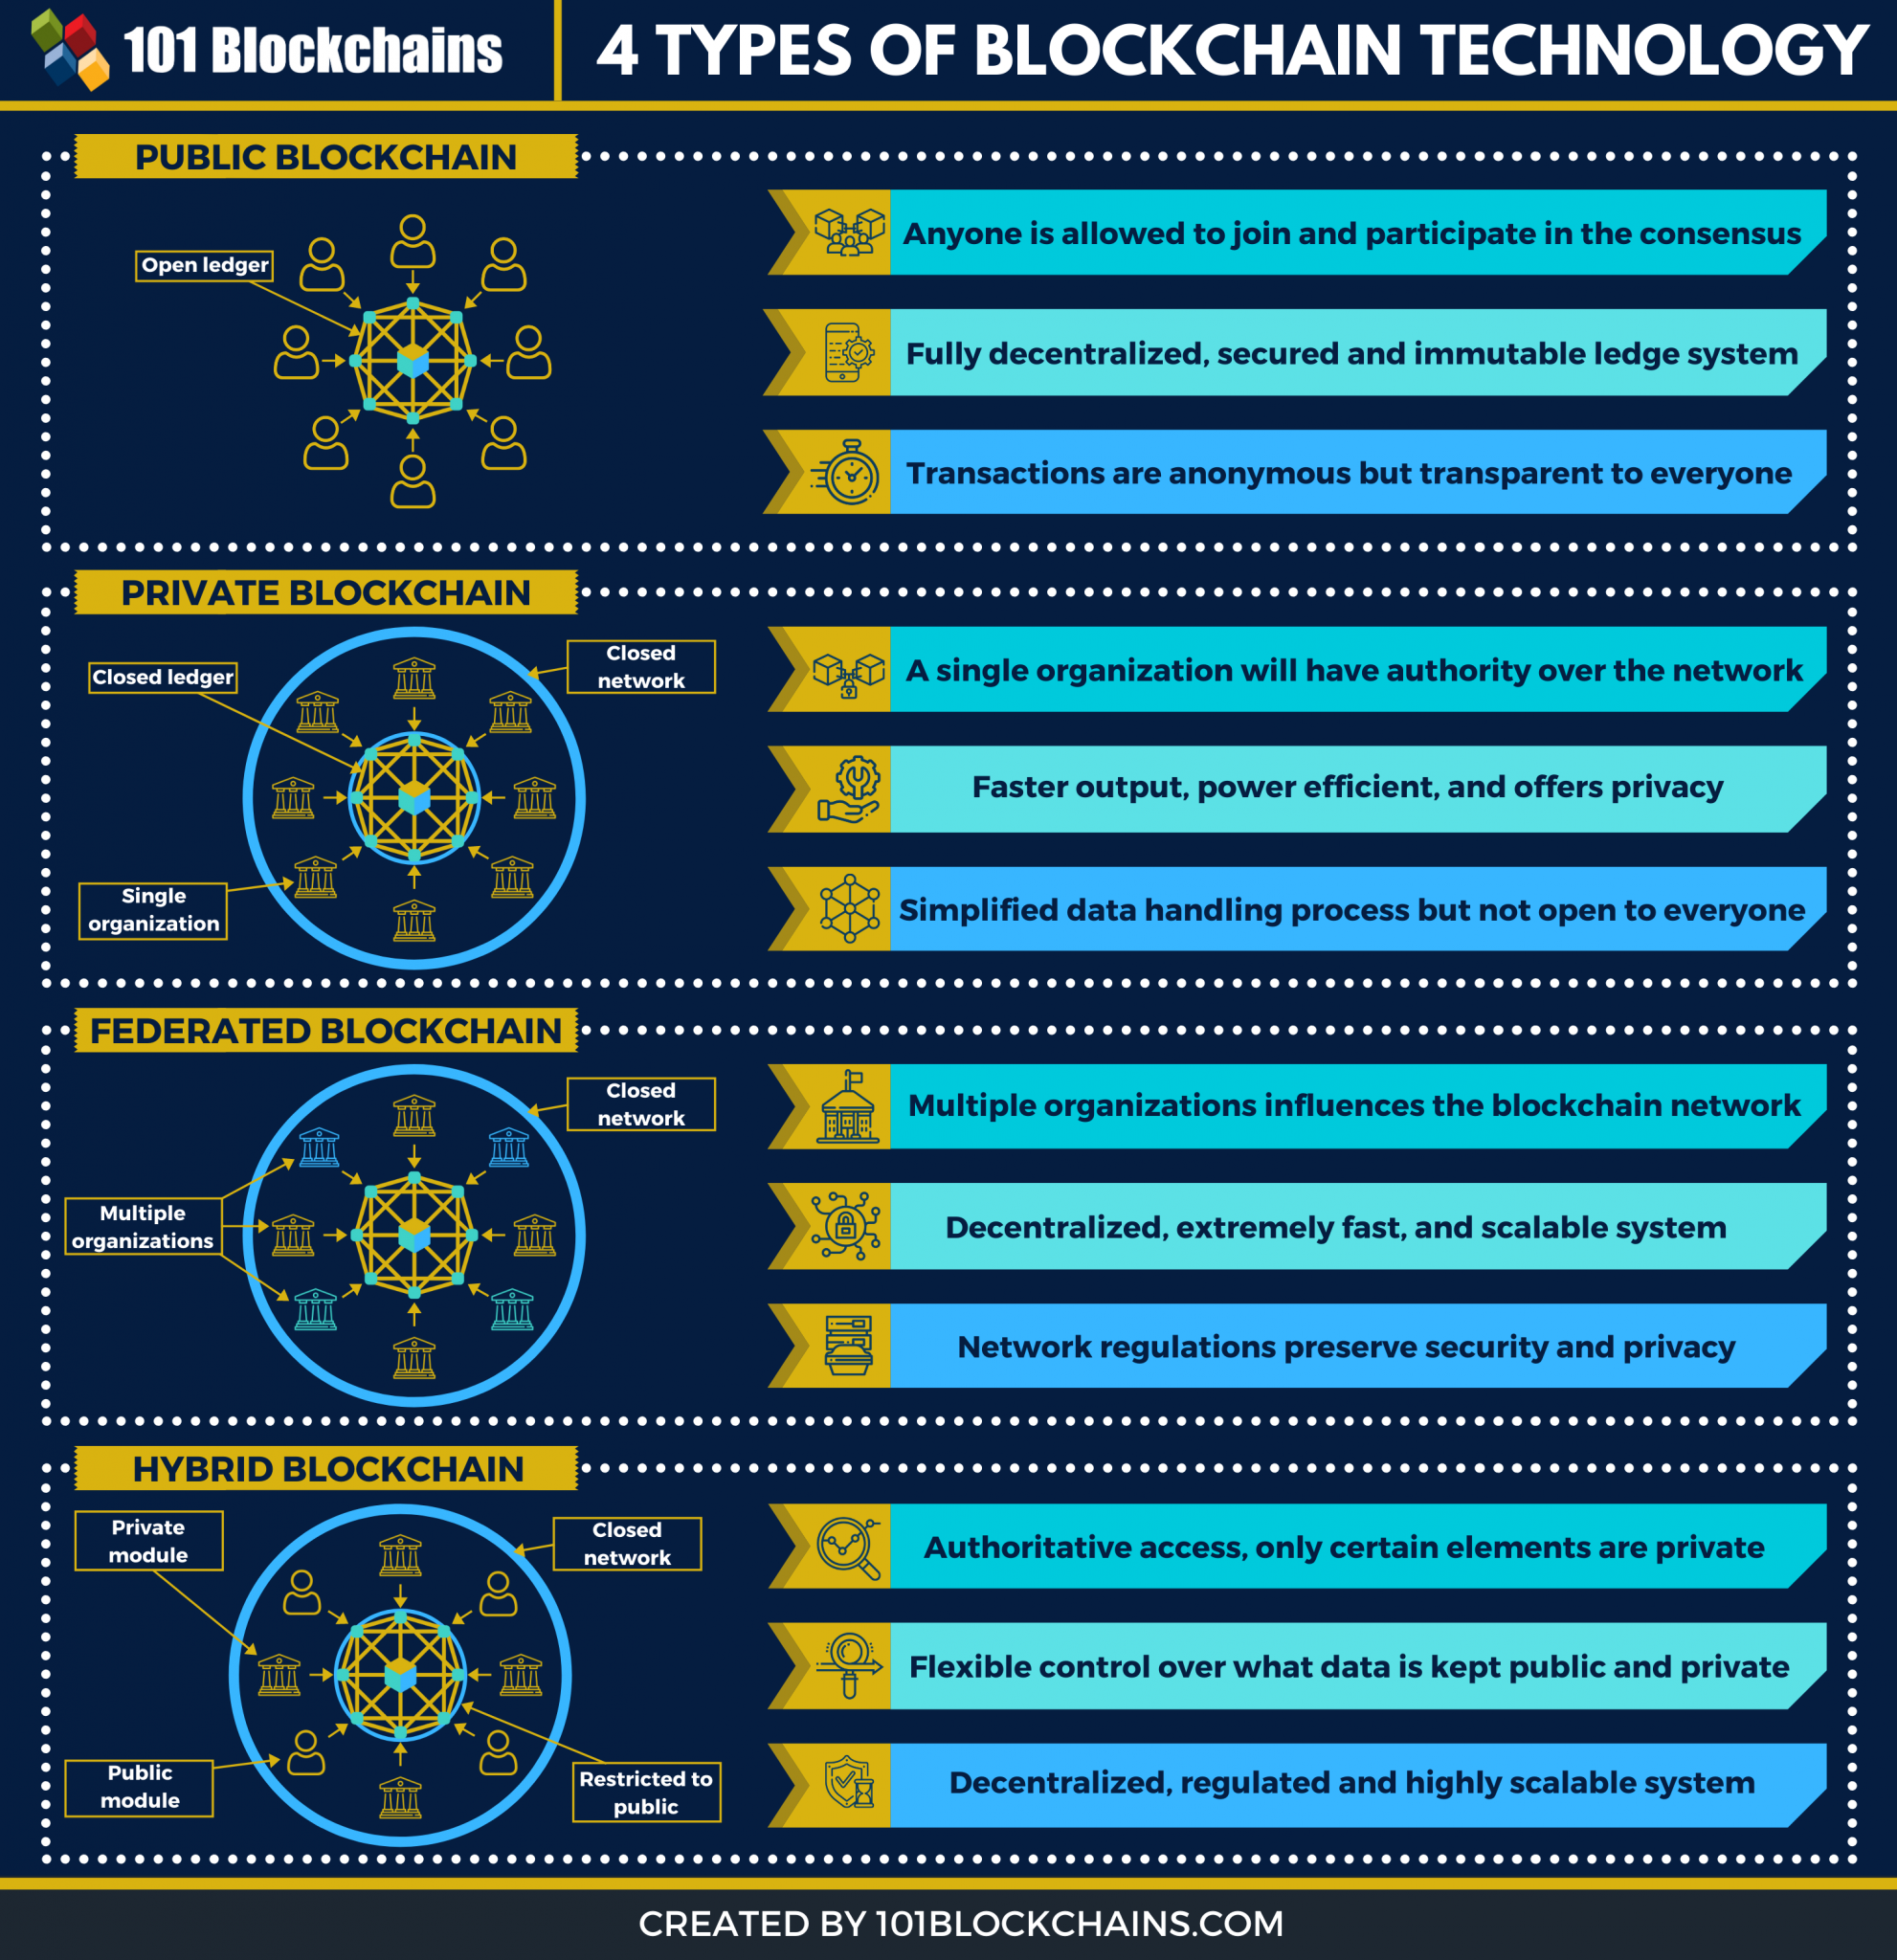
\includegraphics[scale=.2]{recursos/Types-of-Blockchain-Technology-1982x2048.png}}
\caption{Tipos de redes blockchain.}
\label{tipos-BC}
\end{figure}

\begin{enumerate}
\item \textbf{Pública:} En este tipo de redes, no hay ningún sistema de permisos, y cualquier entidad puede acceder a la blockchain y llevar a cabo transacciones. Esto conlleva que la verificación sea muy lenta, debido a los algoritmos utilizados para validar cada transacción, como Proof of Work \cite{POW}. Un ejemplo son las redes Ethereum \cite{ethereum}.
\item \textbf{Privada:} Una red privada funciona normalmente en entornos cerrados, como en el dominio de una compañía, y siempre están gestionadas por una entidad, lo que fuerza cierto grado de centralización. Las redes privadas solo permiten el acceso a entidades selectas, lo que las convierte por defecto en redes permisionadas, de las que hablaremos mas adelante. Por lo demás, su funcionamiento es idéntico al de una red pública. Un ejemplo son las redes Hyperledger Fabric \cite{fabric}.
\item \textbf{Federada/Consorcio:} Las redes federadas tienen partes públicas y partes privadas, y están diseñadas con el objetivo de facilitar la colaboración de varias empresas o entidades en la misma red. A diferencia de las privadas, en las redes federadas el control se comparte entre varias organizaciones, por lo que son mas descentralizadas que las anteriormente mencionadas. Un ejemplo de este tipo de red es Marco Polo.
\item \textbf{Híbrida:} En este tipo de red, se intentan combinar las características de las redes públicas y privadas, con una arquitectura muy maleable, que se puede adaptar a todo tipo de circunstancias, sin dejar de lado aspectos importantes como la transparencia o la seguridad. El acceso sigue estando regulado, pero hay partes públicas y privadas, cosa que depende enteramente de la red en particular. Un ejemplo son las redes Dragonchain.
\end{enumerate}

Además de estos cuatro tipos, existe una característica extra que puede añadirse a estas redes, y es que pueden ser permisionadas o no. Una red permisionada utiliza sistemas de identificación con las entidades que quieren utilizarla, además de asignación de roles para restringir el acceso a ciertas partes de la red a usuarios mas privilegiados. Un ejemplo de red pública permisionada son las basadas en Corda.

\section{Alastria ID}
Alastria ID es el modelo de identidad planteado por el consorcio Alastria, y que se basa en tres pilares fundamentales, siguiendo los principios de la identidad soberana que vimos anteriormente.
\begin{figure}[H]
\centerline{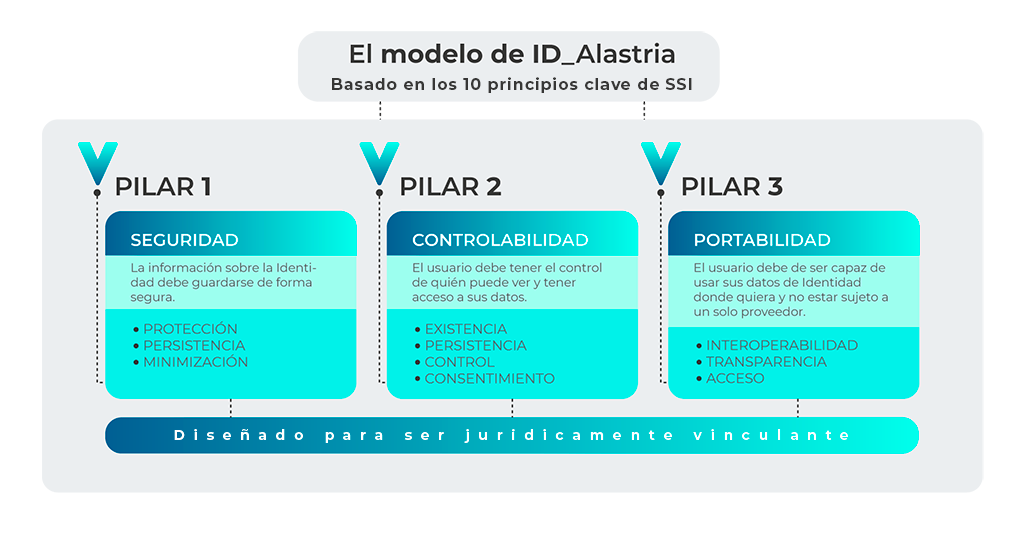
\includegraphics[scale=.5]{recursos/ID-Model-Esp-1.png}}
\caption{Pilares de Alastria ID.}
\label{pilares-alastriaid}
\end{figure}
\begin{enumerate}
    \item \textbf{Seguridad:} La información sobre la identidad se guarda en un \textit{wallet}, una aplicación móvil que aloja los datos en una zona altamente segura del dispositivo.
    \item \textbf{Controlabilidad:} El usuario controla sus datos por completo gracias a que se almacenan en su propio dispositivo, y gracias al uso de las credenciales y la capacidad para revocar su uso en cualquier momento.
    \item \textbf{Portabilidad:} Los datos del usuario siempre están con él gracias a que se guardan en el wallet. Además Alastria ID cuenta con capacidad para recuperar datos en caso de pérdida o robo.
\end{enumerate}
\subsection{Roles}
En el intercambio de credenciales y en todas las operaciones con Alastria ID, cada participante tiene un rol, ya sea una empresa, organización o individuo.
\begin{itemize}
    \item \textbf{Entity/Entidad:} Una entidad representa a una organización o empresa, pero no a un individuo.
    \item \textbf{Issuer/Emisor:} Entidad que tiene la posibilidad de crear credenciales y otorgarlas, ya sea a sujetos o a otras entidades. 
    \item \textbf{Service Provider/Proveedor de Servicios:} Entidad que proporciona servicios a sujetos o a otras entidades, utilizando opcionalmente credenciales. Son las encargadas de crear solicitudes de presentación y de recibir presentaciones con las credenciales requeridas para sus servicios.
    \item \textbf{Subject/Sujeto:} Persona física que se beneficia de las entidades, ya sea recibiendo credenciales de los emisores o servicios de los proveedores de servicio. Es propietario de un wallet de identidad, donde guarda sus credenciales y mediante el que recibe y envía solicitudes de presentación y presentaciones, respectivamente.
\end{itemize}
Cabe destacar que una entidad puede ser emisor y proveedor de servicio al mismo tiempo, e interactuar con otras entidades y recibir credenciales y servicios como si fuese un sujeto.
\subsection{DID}
DID significa \textit{Decentralized Identifier}, y puede referirse a cualquier tipo de sujeto (por ej.: personas, empresas, modelos de datos, entidades abstractas, etc...), están diseñados para ser completamente independientes de registros centralizados, y son capaces de demostrar que su propietario tiene el control sobre el elemento representado, sin necesidad de actores externos.

En Alastria ID, los DIDs se usan para representar a las entidades y a los sujetos, y tienen el siguiente formato \cite{did-credentials-presentations}:
\begin{verbatim}
did                     = "did:ala:" red ":" string-identificador
red                     = ("quor" / "fabr") ":" id-red
string-identificador    = depende de la red
\end{verbatim}
La definición de los componentes:
\begin{itemize}
    \item \textbf{ala:} Significa que este DID es de Alastria ID
    \item \textbf{red:} Especifica la tecnología que utiliza la red blockchain a la que pertenece el DID. Actualmente se utiliza ``quor'' para la red Quorum, pero próximamente se podrá utilizar ``fabr'' para la red Fabric.
    \item \textbf{id-red:} Representa la red blockchain específica, por ejemplo ``redt''.
    \item \textbf{string-identificador:} Depende de la red a la que pertenezca el DID. En la red disponible actual, que es la de Quorum, es la dirección Ethereum del "Proxy Contract" que representa al Alastria ID de la entidad. Su funcionamiento en la red Fabric se tratará en un apartado posterior.
\end{itemize}
\clearpage
\subsection{PSMHashes}
Tanto las credenciales como las presentaciones se representan e identifican mediante los llamados \acrshort{psmhash}. Un \acrshort{psmhash} es el hash de la suma del \acrshort{did} y la credencial o presentación. Cada credencial o presentación tiene dos \acrshort{psmhash}es, uno formado con el DID del emisor y otro con el DID del sujeto.
\begin{figure}[H]
\centerline{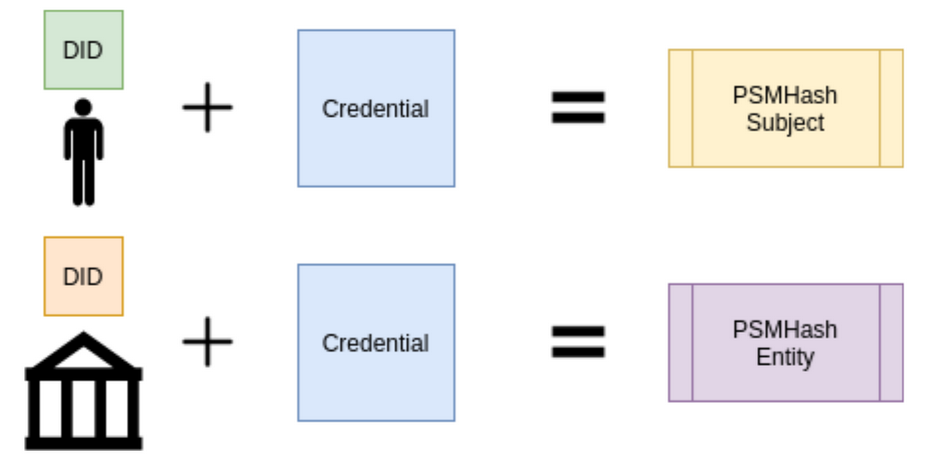
\includegraphics[scale=.7]{recursos/psmhashes.png}}
\caption{Estructura de los PSMHashes.}
\label{psmhashes}
\end{figure}
\subsection{Artefactos}
\subsubsection{Definición}
Los artefactos de Alastria son objetos \acrshort{jwt}, que tienen tres partes, \textit{header}, o cabecera, \textit{payload}, o cuerpo y \textit{signature}, o firma.
Cada una de estas partes se representa cifrada en Base64, y se unen mediante puntos (xxxx.yyyy.zzzz).
\subsubsection*{Cabecera}
Una cabecera esta formado por cuatro campos:
\begin{itemize}
    \item \textbf{alg:} Algoritmo utilizado para hashear el token
    \item \textbf{typ:} Tipo de token
    \item \textbf{kid:} Identificador de la clave pública utilizada. Opcional.
    \item \textbf{jwk:} Clave pública utilizada. Opcional.
\end{itemize}
Un ejemplo:
\begin{verbatim}
{
    "alg": "ES256K",
    "typ": "JWT",
    "kid": "did:ala:quor:redt:QmeeasCZ9jLbX...ueBJ7d7csxhb#keys-1",
    "jwk": "0x2e507af01167c98a6acc...83cf9779e4ea98d13df2833f3767"
}
\end{verbatim}
\subsubsection*{Cuerpo}
Depende del tipo de artefacto, en Alastria son \acrshort{at}, \acrshort{as} y \acrshort{aic}. También se incluyen las credenciales, solicitudes de presentación y presentaciones.
\subsubsection*{Firma}
La firma debe utilizar el algoritmo especificado en la cabecera, e incluye todo el \acrshort{jwt} a la hora de firmar.\\

En los siguientes apartados solo se describirá la parte del cuerpo de cada uno de los artefactos, puesto que tanto cabecera y firma utilizan siempre el mismo formato.
\subsubsection{JWTs de Alastria}
Hay tres objetos principales \cite{alastria-artifacts} utilizados en Alastria para la creación de identidades, la emisión de credenciales y la autenticación.
\subsubsection*{Alastria Token}
Se utiliza en cuatro flujos diferentes; la creación de identidades, la autenticación, la emisión de credenciales y en el envío de presentaciones.
Tiene seis campos obligatorios:
\begin{itemize}
    \item \textbf{iss:} DID del emisor del AT.
    \item \textbf{gwu:} URL del \textit{gateway} del que envía.
    \item \textbf{cbu:} URL de \textit{callback} a la que se debe responder.
    \item \textbf{ani:} Alastria Network ID. Identificador de la red de Alastria ID correspondiente.
    \item \textbf{iat:} Issued At. Tiempo de emisión del token.
    \item \textbf{exp:} Tiempo de expiración del token.
\end{itemize}
Tambien tiene cuatro campos opcionales:
\begin{itemize}
    \item \textbf{type:} Tipo de token (en este caso sería ``AlastriaToken'').
    \item \textbf{nbf:} NotBefore. Tiempo a partir del cual este token es válido.
    \item \textbf{jti:} Identificador único del JWT.
    \item \textbf{mfau:} \acrshort{mfau} URL. URL opcional para implementar autenticación multifactor.
\end{itemize}
Un ejemplo:
\begin{verbatim}
{
  "type": ["AlastriaToken","US12"]
  "nbf": 1587712704319,
  "gwu": "http://url/rpc",
  "cbu": "http://url/loginAID",
  "iss": "did:ala:quor:redT:3235c170482ff9ca250fb2a3b83468cb605f6a4c",
  "exp": 1587799104319,
  "ani": "redT",
  "iat": 1587712704319,
  "jti": "ze298y42sba",
  "mfau": "http://url/mfa_server"
}
\end{verbatim}
\subsubsection*{Alastria Session}
Su uso varía entre la autenticación de un usuario y la emisión de credenciales, y se distingue entre ellos añadiendo la historia de usuario correspondiente al campo \textit{type}.
Tiene cuatro campos obligatorios:
\begin{itemize}
    \item \textbf{@context:} URLs con la especificación del token, debe ser al menos\\ ``https://alastria.github.io/identity/artifacts/v1''.
    \item \textbf{type:} Tipo de token (en este caso sería ``AlastriaSession'').
    \item \textbf{iss:} DID del emisor del token. 
    \item \textbf{alastriaToken:} \acrshort{at} en formato \acrshort{jwt}. Es el AT al que este AS responde.
\end{itemize}
También puede tener cuatro campos opcionales mas; jti, iat, exp y nbf, que son los mismos que en el \acrshort{at} y en el \acrshort{aic}.
Un ejemplo de Alastria Session:
\begin{verbatim}
{
  "jti": "ze298y42sba"  
  "@context": ["https://alastria.github.io/identity/artifacts/v1"],
  "type": ["AlastriaSession","US211"]
  "iss": "did:ala:quor:redT:07dba616e17a45fca5cfc999a584180e45353aa9",
  "iat": 1587712763,
  "exp": 1563783392,
  "nbf": 1563783392,
  "alastriaToken": "eyJ0..4ea8",
}
\end{verbatim}
\subsubsection*{Alastria Identity Creation}
Es el objeto que envían los sujetos desde el \textit{wallet} para registrar un nuevo Alastria ID, completando así el ultimo paso de la creación de identidad.
Tiene cinco campos obligatorios:
\begin{itemize}
    \item \textbf{@context:} URLs con la especificación del token, debe ser al menos\\ ``https://alastria.github.io/identity/artifacts/v1''.
    \item \textbf{type:} Tipo de token (en este caso sería ``AlastriaIdentityCreation'').
    \item \textbf{createAlastriaTX:} Transacción en hexadecimal de creación de Alastria ID, firmada por el sujeto.
    \item \textbf{alastriaToken:} \acrshort{at} en formato \acrshort{jwt}. Es el \acrshort{at} original al que este \acrshort{aic} responde. Cabe destacar que no está firmado, ya que está dentro de un \acrshort{aic} firmado.
    \item \textbf{publicKey:} Clave pública del sujeto en hexadecimal. 
\end{itemize}
También puede tener cuatro campos opcionales mas; jti, iat, exp y nbf, que son los mismos que en el \acrshort{at} y en el \acrshort{as}.
Un ejemplo:
\begin{verbatim}
{
  "@context": ["https://alastria.github.io/identity/artifacts/v1"],
  "type": ["AlastriaIdentityCreation","US12"],
  "createAlastriaTX":"0xf9...",
  "alastriaToken":"ey...",
  "publicKey":"0x2e...",
  "jti": "ze298y42sba",
  "iat": 1587712763,
  "exp": 1563783392,
  "nbf": 1563783392
}
\end{verbatim}
\subsubsection{Intercambio de credenciales}
Los objetos dedicados al intercambio de credenciales \cite{did-credentials-presentations} siguen el mismo formato \acrshort{jwt} de los artefactos de Alastria, y comparten la misma cabecera, que tiene los siguientes campos obligatorios:
\begin{itemize}
    \item \textbf{typ:} Tipo del formato, siempre es ``JWT''.
    \item \textbf{alg:} Algoritmo utilizado en la firma del \acrshort{jwt}, siempre es ES256K.
\end{itemize}
También tiene otros dos campos opcionales:
\begin{itemize}
    \item \textbf{kid:} Identificador de la clave pública usada para firmar el \acrshort{jwt}. En Alastria es el \acrshort{did} de la clave pública seguido por ``\#keys-1''.
    \item \textbf{jwk:} Clave pública usada para firmar el \acrshort{jwt}.
\end{itemize}
Un ejemplo:
\begin{verbatim}
{
    "alg": "ES256K",
    "typ": "JWT",
    "kid": "did:ala:quor:redt:3eabc53a851fc5...1cc4b2b5d1#keys-1",
    "jwk": "0x2e507af01167c98a6accc0c...ea98d13df2833f3767"
}
\end{verbatim}
El apartado de firma de estos \acrshort{jwt}s es siempre el mismo, expuesto en una sección anterior.
En los siguientes apartados se describirá la parte del cuerpo de los \acrshort{jwt}s de intercambio de credenciales. Todos los campos referentes a tiempo están en formato ``NumericDate'' de \acrshort{json}.
\subsubsection*{Credencial}
Las credenciales contienen datos sobre un sujeto o entidad, son otorgadas por un emisor y se entregan a los proveedores de servicio mediante presentaciones. 
Tienen seis campos simples y uno complejo, que contiene tres campos como mínimo:
\begin{itemize}
    \item \textbf{jti:} Identificador único de la credencial. Opcional.
    \item \textbf{iss:} \acrshort{did} de la entidad emisora de la credencial. Obligatorio.
    \item \textbf{sub:} \acrshort{did} del sujeto al que se le ha emitido la credencial. Opcional.
    \item \textbf{iat:} Tiempo de emisión de la credencial. Obligatorio.
    \item \textbf{exp:} Tiempo de expiración de la credencial. Opcional.
    \item \textbf{nbf:} Tiempo a partir del cual esta credencial es válida. Opcional.
    \item \textbf{vc:} \textit{Verifiable Credential}. Es el objeto que tiene la información en si de la credencial.
    \begin{itemize}
        \item \textbf{@context:} Un array de URLs con información sobre la definición de la credencial. Como mínimo debe contener \\
        ``https://alastria.github.io/identity/credentials/v1'' y \\``https://www.w3.org/2018/credentials/v1''.
        \item \textbf{type:} Un array con los tipos de credencial. Como mínimo debe contener ``VerifiableCredential'' y ``AlastriaVerifiableCredential''.
        \item \textbf{levelOfAssurance:} Es el nivel de confianza en la credencial. Está basado en los niveles de confianza de \acrshort{eidas}. Sus valores posibles son ``Self'', ``Low'', ``Substantial'' y ``High''. Se suele encontrar dentro de un campo llamado ``credentialSubject'', que contiene los datos que representa la credencial. Opcional.
    \end{itemize}
\end{itemize}
Un ejemplo:
\begin{verbatim}
{
  "jti": "https://www.oneweb.com/alastria/credentials/3732",
  "iss": "did:alastria:quorum:redt:c5039eae214608f...aeea381ccb5d1",
  "sub": "did:alastria:quorum:redt:3eabc53a851fc50...acf8cc4b2b5d1",
  "iat": 1525465044,
  "exp": 1530735444,
  "nbf": 1525465044,
  "vc": {
    "@context": [
      "https://www.w3.org/2018/credentials/v1",
      "https://alastria.github.io/identity/credentials/v1",
      "https://universities.io/examples/v1"
    ],
    "type": ["VerifiableCredential","AlastriaVerifiableCredential", 
            "UniversityDegreeCredential"],
    "credentialSubject": {
      "levelOfAssurance": 0,
      "degree": {
        "type": "BachelorDegree",
        "name": "Bachelor of Science and Arts"
      }
    }
  }
}
\end{verbatim}
\subsubsection*{Presentation/Presentación}
Las presentaciones contienen una o más credenciales, y son el medio por el que los proveedores de servicio reciben las credenciales necesarias de entidades o sujetos. Son la respuesta a las solicitudes de presentación.
Tienen siete campos simples y uno complejo, que contiene cinco campos mas:
\begin{itemize}
    \item \textbf{jti:} Identificador único de la presentation. Opcional.
    \item \textbf{iss:} \acrshort{did} del sujeto o entidad que ha creado la presentation. Obligatorio.
    \item \textbf{aud:} \acrshort{did} de la entidad a la que va destinada la presentation. Obligatorio.
    \item \textbf{iat:} Tiempo de creación de la presentación. Obligatorio.
    \item \textbf{exp:} Tiempo de expiración de la presentación. Opcional.
    \item \textbf{nbf:} Tiempo a partir del cual la presentación es válida. Opcional.
    \item \textbf{jtipr:} Identificador único de la solicitud de presentación asociada a la presentación. Opcional.
    \item \textbf{vp:} \textit{Verifiable Presentation}. Es el objeto que contiene la información de la presentación en si. Contiene cinco campos obligatorios.
    \begin{itemize}
        \item \textbf{@context:} Un array de URLs con información sobre la definición de la credencial. Como mínimo debe contener\\
        ``https://alastria.github.io/identity/credentials/v1'' y \\
        ``https://www.w3.org/2018/credentials/v1''.
        \item \textbf{type:} Un array con los tipos de presentación. Como mínimo debe contener ``VerifiablePresentation'' y ``AlastriaVerifiablePresentation''.
        \item \textbf{procHash:} Es el hash de un documento que describe el propósito de las credenciales que se envían. 
        \item \textbf{procUrl:} Es la URL donde se aloja un documento que describe el propósito de las credenciales que se envían. 
        \item \textbf{verifiableCredential:} Es un array de credenciales requeridas en formato \acrshort{jwt}.
    \end{itemize}
\end{itemize}
Un ejemplo:
\begin{verbatim}
{
  "jti": "https://www.empresa.com/alastria/credentials/3732",
  "iss": "did:alastria:quorum:redt:3eabc53...924a381cc4b2b5d1",
  "aud": "did:alastria:quorum:redt:3eabc53...924a381cc4b2b5d1",
  "iat": 1525465044,
  "exp": 1530735444,
  "nbf": 1525465044,
  "jtipr": "metrovacesa/alastria/presentationrequest/7864",
  "vp": {
    "@context": [
      "https://www.w3.org/2018/credentials/v1",
      "https://alastria.github.io/identity/credentials/v1",
    ],
    "type": ["VerifiablePresentation", "AlastriaVerifiablePresentation"],
    "procHash": "H398sjHd...kldjUYn475n",
    "procUrl": "https://www.empresa.com/alastria/businessprocess/4583",
    "verifiableCredential": [{ ... }]
  }
}
\end{verbatim}
\subsubsection*{Presentation Request/Solicitud de presentación}
Las solicitudes de presentación son el método que tienen los proveedores de servicio de solicitar las credenciales necesarias a los sujetos o entidades, con el fin de otorgar un servicio.
Tienen cinco campos simples y uno complejo, que a su vez contiene seis campos:
\begin{itemize}
    \item \textbf{jti:} Identificador único de la solicitud de presentación. Opcional.
    \item \textbf{cbu:} URL de \textit{callback} del proveedor de servicio. Obligatorio.
    \item \textbf{iss:} \acrshort{did} del proveedor de servicio que ha creado la solicitud de presentación. Obligatorio.
    \item \textbf{iat:} Tiempo de creación de la solicitud de presentación. Obligatorio.
    \item \textbf{exp:} Tiempo de expiración de la solicitud de presentación. Opcional.
    \item \textbf{pr:} Objeto que contiene los datos de la solicitud de presentación. Tiene cinco campos simples y uno complejo, que a su vez contiene cuatro campos:
    \begin{itemize}
        \item \textbf{@context:} Un array de URLs con información sobre la definición de la solicitud de presentación. Como mínimo debe contener\\
        ``https://alastria.github.io/identity/credentials/v1'' y \\
        ``https://www.w3.org/2018/credentials/v1''. Obligatorio.
        \item \textbf{type:} Un array con los tipos de solicitud de presentación. Como mínimo debe contener ``VerifiablePresentationRequest'' y\\ ``AlastriaVerifiablePresentationRequest". Obligatorio.
        \item \textbf{procHash:} Es el hash de un documento que describe el propósito de las credenciales que se solicitan. Obligatorio.
        \item \textbf{procUrl:} Es la URL donde se aloja un documento que describe el propósito de las credenciales que se solicitan. Obligatorio. 
        \item \textbf{procDesc:} Descripción del propósito de las credenciales que se solicitan. Opcional.
        \item \textbf{data:} Es un array en el que cada objeto representa una credencial solicitada. Tiene tres campos obligatorios y uno opcional:
        \begin{itemize}
            \item \textbf{@context:} Un array de URLs con información sobre la credencial. Obligatorio.
            \item \textbf{levelOfAssurance:} Es el nivel de confianza mínimo que se requiere de la credencial. Está basado en los niveles de confianza de \acrshort{eidas}. Sus valores posibles son ``Self'', ``Low'', ``Substantial'' y ``High''. Opcional.
            \item \textbf{required:} Es un booleano que especifica si la credencial es obligatoria o no. Obligatorio.
            \item \textbf{field\_name:} Nombre de la credencial requerida. Obligatorio.
        \end{itemize}
    \end{itemize}
\end{itemize}
Un ejemplo:
\begin{verbatim}
{
  "jti": "metrovacesa/alastria/presentationrequest/7864",
  "iss": "did:alastria:quorum:testnet1:3eabc53a851f...a381cc4b2b5d1",
  "iat": 1525465044,
  "exp": 1530735444,
  "nbf": 1525465044,
  "cbu": "https://www.metrovacesa.com/alastria/presentation?jtipr=7864"

  "pr": {
    "@context": [
      "https://www.w3.org/2018/credentials/v1",
      "https://alastria.github.io/identity/credentials/v1"
    ],
    "type": ["VerifiablePresentationRequest", 
        "AlastriaVerifiablePresentationRequest"],
    "procHash": "H398sjHd...kldjUYn475n",
    "procUrl": "https://www.ejemplo.com/alastria/businessprocess/4583",
    "procDesc": "Descripción corta del propósito de la PR",
    "data": [
      {
        "@context": ["https://alastria.github.io/identity/covid/v1"],
        "levelOfAssurance": 3,
        "required": true,
        "field_name": "covid_test",
      },
      {
        "@context": ["https://alastria.github.io/identity/examples/v1"],
        "levelOfAssurance": 2,
        "required": true,
        "field_name": "phone_number",
      }
    ]
  }
}
\end{verbatim}

\clearpage
\section{Hyperledger Fabric}
Hyperledger Fabric es una plataforma \acrshort{dlt} open source creada por Linux Foundation, y diseñada con el uso empresarial en mente, gracias a una arquitectura altamente modular y configurable, y que soporta smart contracts codificados en lenguajes de programación generales, como Java, Go o Node.js.
Las redes de Hyperledger Fabric son privadas permisionadas, lo que significa que los miembros requieren de autenticación para hacer uso de ellas, y lo que también implica que no hay necesidad de algoritmos de consenso pesados como \acrshort{pow} \cite{fabric-simple}.
En los siguientes apartados se describirán los componentes principales del modelo de Hyperledger Fabric.
\subsection{Nodos}
Una red Fabric está compuesta principalmente por uno o más nodos, que pueden ser de dos tipos, peers u orderers.
\subsubsection{Peers}
Los \textit{peers} son el elemento mas importante de una red Fabric, puesto que tanto los \textit{ledgers} como los \textit{chaincodes} se despliegan en ellos. Cada \textit{peer} puede contener tantas instancias de distintos \textit{ledgers} como se desee, así como cualquier cantidad de \textit{chaincodes} que accedan a ellos.
\begin{figure}[H]
\centerline{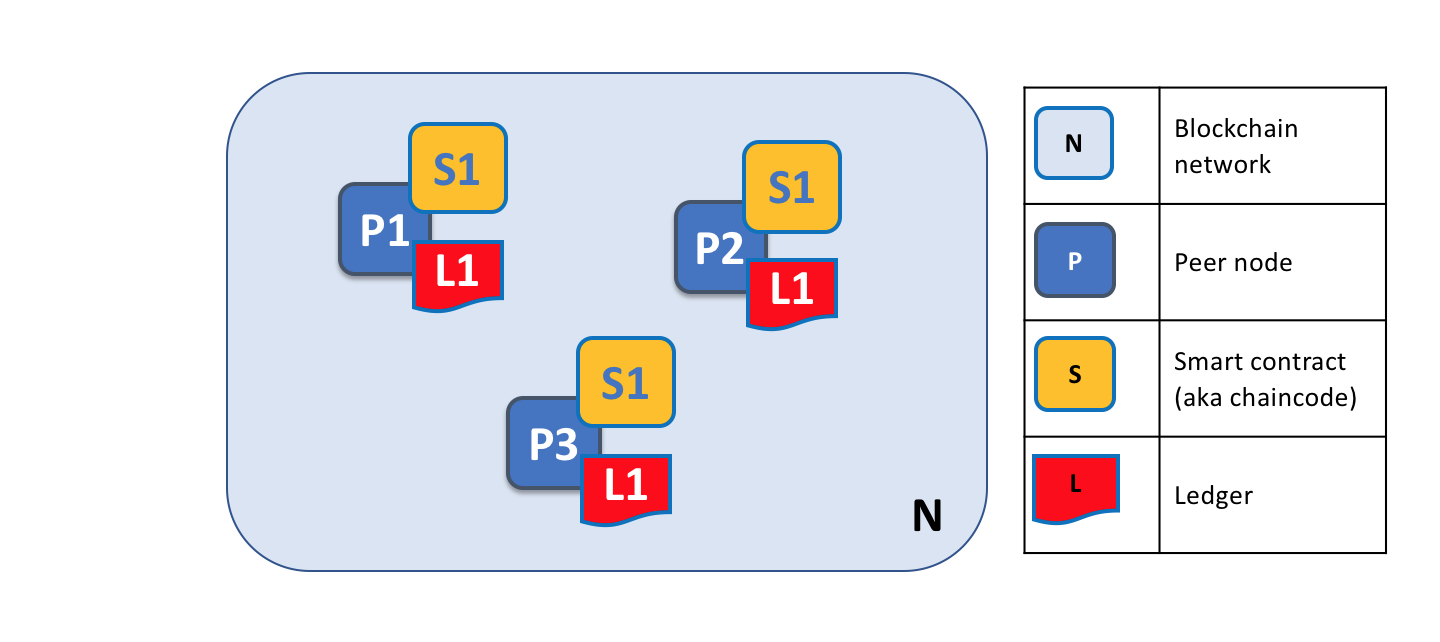
\includegraphics[scale=0.4]{recursos/peers.png}}
\caption{Red Fabric básica.}
\label{peers-network}
\end{figure}
Los \textit{peers} también exponen varias APIs para que aplicaciones externas puedan interactuar con la blockchain. Esto se hace mediante el uso de transacciones, y aquí es donde entran en juego los nodos \textit{orderer}, que se describirán en el siguiente apartado.
En la figura anterior, se puede observar que todos los nodos tienen instancias del mismo \textit{ledger} (L1), con sus correspondientes \textit{chaincodes} (S1). Esto es debido a que todos los nodos deben estar sincronizados para que sea posible una implementación descentralizada.
\begin{figure}[h]
\centerline{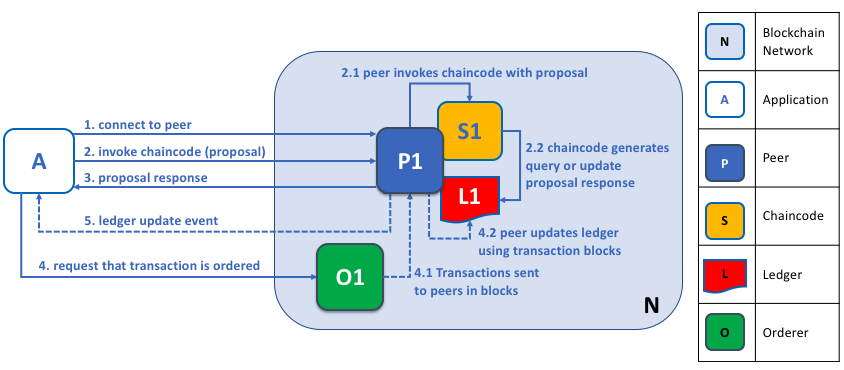
\includegraphics[scale=0.6]{recursos/peers-aplicacion.png}}
\caption{Interacción de una aplicación externa con la red.}
\label{peers-application}
\end{figure}
\clearpage
\subsubsection{Orderers}
Los nodos \textit{orderer} se encargan de ordenar las transacciones y de crear un bloque con ellas, para después enviarlo de vuelta a los \textit{peers} y que los \textit{ledgers} de todos ellos se mantengan sincronizados. Los \textit{orderers} son necesarios en redes con mas de un \textit{peer}, ya que, al generarse varias transacciones es necesario saber su orden para mantener las blockchains coordinadas.
\begin{figure}[H]
\centerline{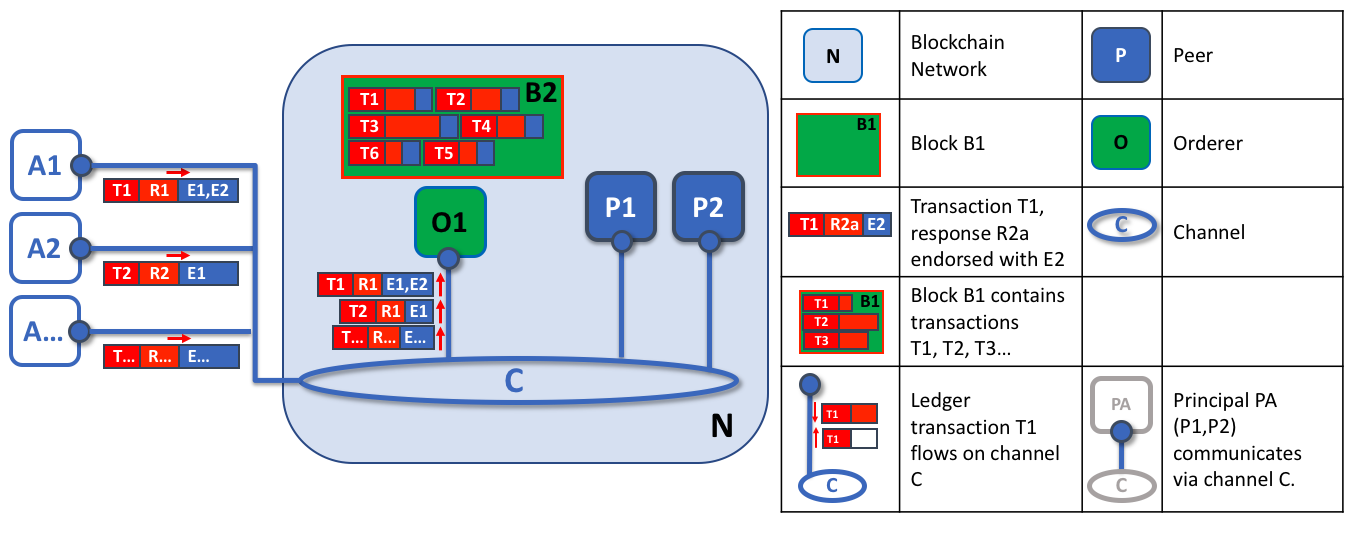
\includegraphics[scale=0.4]{recursos/orderers.png}}
\caption{Creación de bloques por parte del orderer.}
\label{orderers}
\end{figure}
En el diagrama anterior, se puede observar como las transacciones y sus respuestas ya validadas por los peers (T1, R1, validadas por E1 y E2) salen de las aplicaciones y van al \textit{orderer} (O1), que las ordena y las introduce en un bloque (B2). Este bloque se envía a todos los \textit{peers} para que actualicen el estado de sus \textit{ledgers} con la información de las transacciones.
Nótese que todos los elementos están conectados en el diagrama a un \textit{channel}, o \textit{channel}, que se describirá en el siguiente apartado.
\clearpage
\subsection{Channels/Canales}
Los \textit{channels}, o canales, son un mecanismo que se utiliza para que los componentes de una red Fabric puedan interactuar de forma privada entre ellos. Un peer puede formar parte de varios \textit{channels}, y cada \textit{channel} tiene sus propias reglas y configuración de acceso. Un \textit{channel} solo puede tener un ledger.
\begin{figure}[H]
\centerline{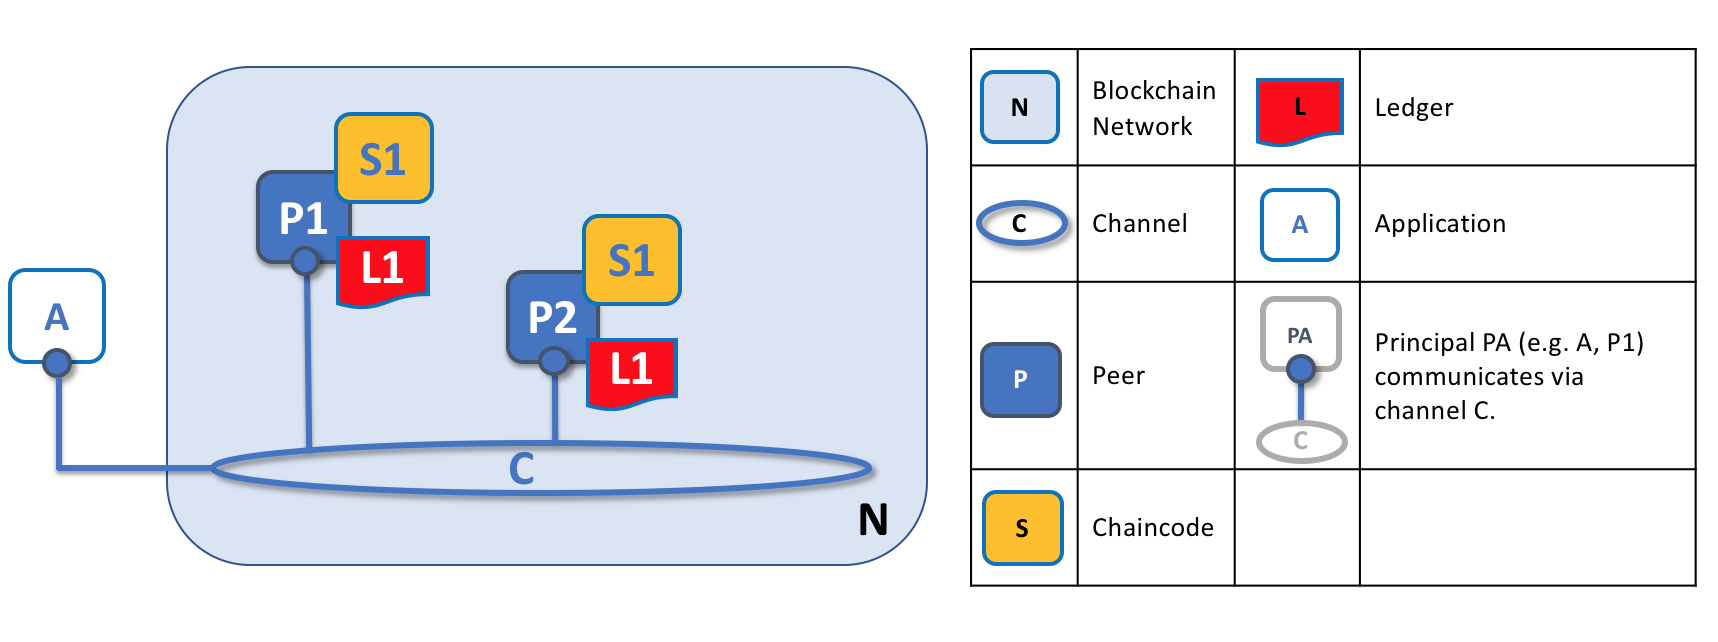
\includegraphics[scale=0.3]{recursos/canales.png}}
\caption{Red simple con un channel y dos peers.}
\label{canales}
\end{figure}
\subsection{Ledger}
En Fabric, un \textit{ledger} contiene la información sobre los objetos, y está compuesto de dos partes, la blockchain y el \textit{world state} (o \textit{state database}).
\begin{figure}[H]
\centerline{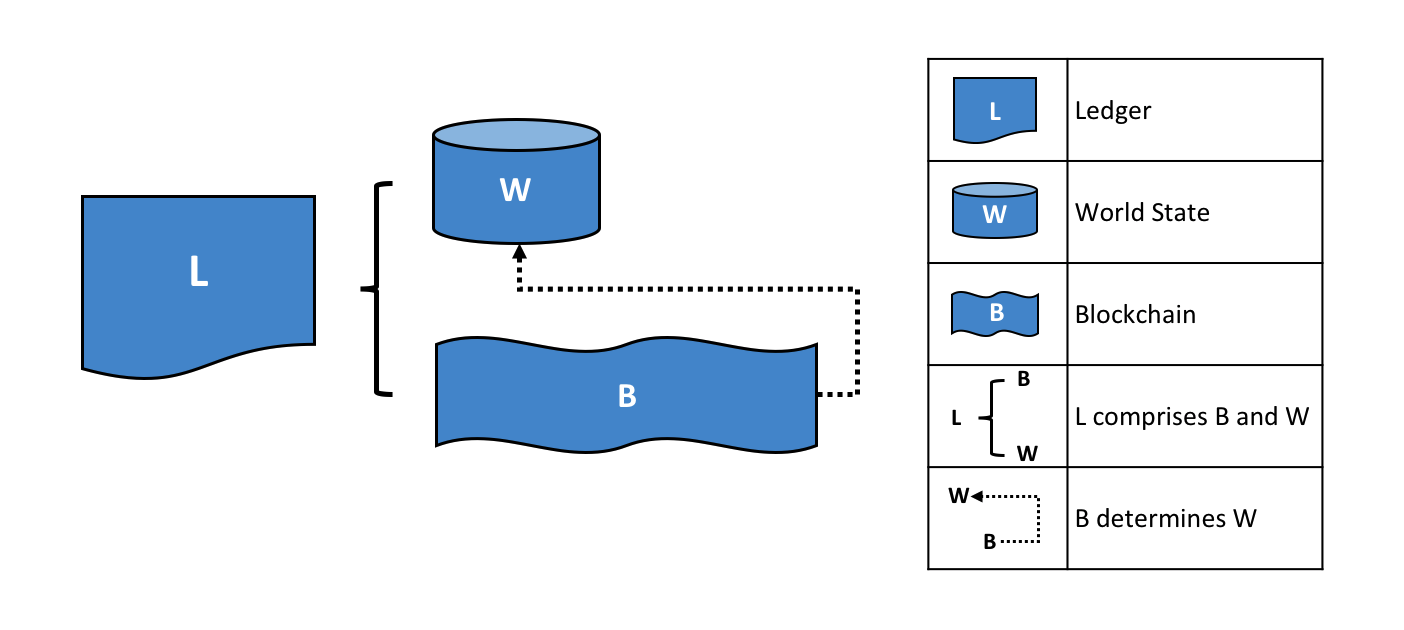
\includegraphics[scale=0.35]{recursos/ledger-partes.png}}
\caption{Un ledger y sus partes.}
\label{ledger}
\end{figure}
\subsubsection{World State/State Database}
El \textit{world state} o \textit{state database} guarda el valor de los objetos en formato clave-valor, además de controlar la versión de cada objeto individualmente.
\begin{figure}[H]
\centerline{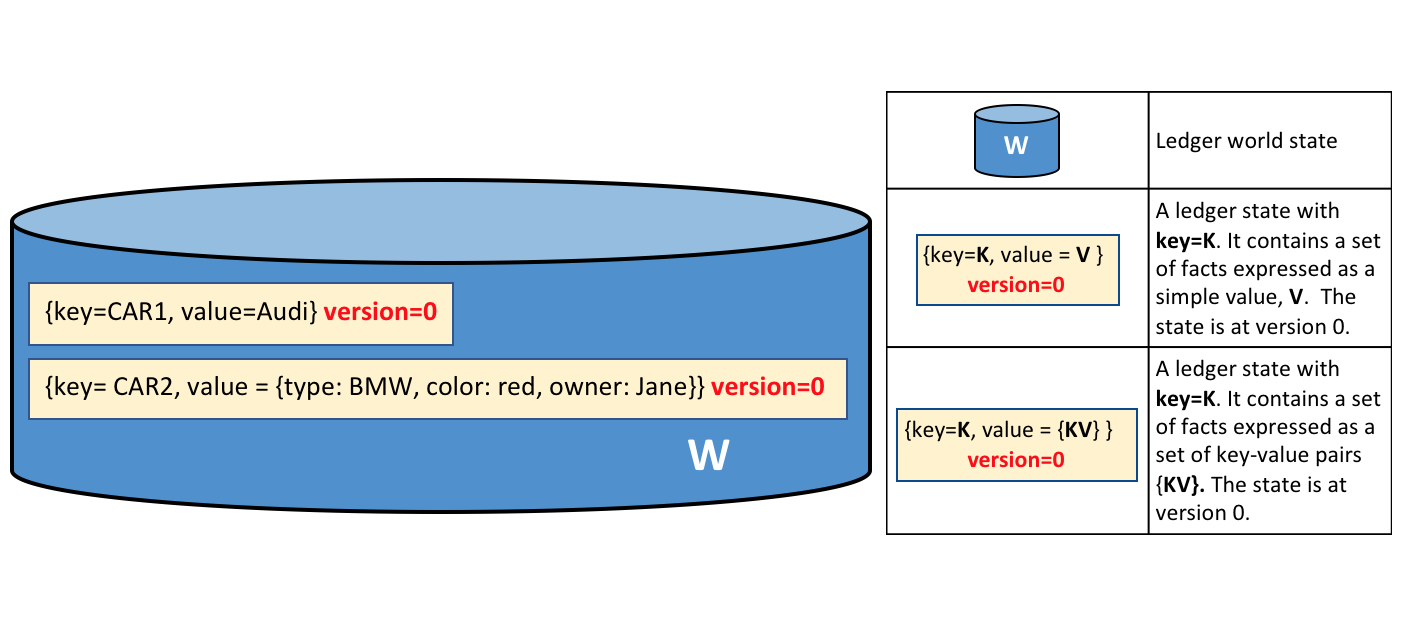
\includegraphics[scale=0.3]{recursos/world-state.png}}
\caption{Componentes de un world state típico.}
\label{world-state}
\end{figure}
En el diagrama se puede observar que los valores de los objetos pueden ser tanto simples como complejos.
El \textit{world state} es en realidad una base de datos, con todas las ventajas que eso conlleva. Hay distintos tipos de bases de datos disponibles, con diferentes características para diferentes proyectos.\\
La funcionalidad principal del \textit{world state} es almacenar todos los cambios en los estados del mundo, realizados por las transacciones, para que el acceso a estos sea lo mas cómodo y eficiente posible. Esto significa que el \textit{world state} es un reflejo de la blockchain, y puede regenerarse a partir de ella en cualquier momento.
\clearpage
\subsubsection{Blockchain}
La parte blockchain del \textit{ledger} es un registro histórico de todos los estados del \textit{ledger}, y está estructurada como una cadena de bloques, donde cada bloque contiene una o mas transacciones ordenadas, que contienen cambios sobre el \textit{world state}.\\
La blockchain esta implementada mediante un archivo, a diferencia del \textit{world state}.
\begin{figure}[H]
\centerline{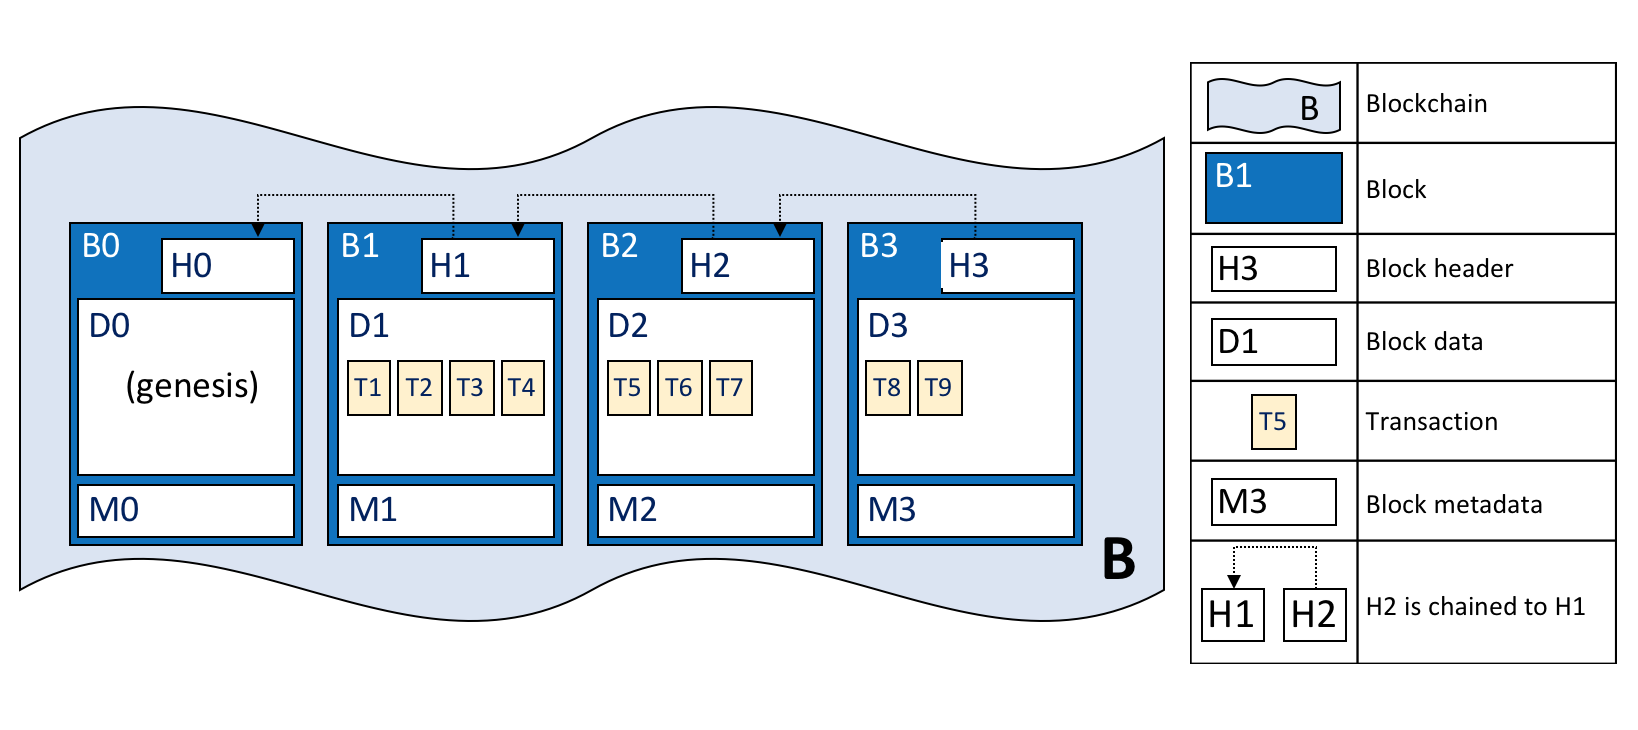
\includegraphics[scale=0.3]{recursos/blockchain-ledger.png}}
\caption{Estructura básica de una blockchain en Fabric.}
\label{blockchain}
\end{figure}
En la figura anterior, se puede observar como todos los bloques tienen tres partes, la cabecera, las transacciones y los metadatos. La cabecera es un hash formado por todas las transacciones del bloque, asi como la cabecera del bloque anterior. Esto genera una conexión inmutable entre todos los bloques, lo que da su nombre a la blockchain. En el cuerpo del bloque se encuentran las transacciones ordenadas por el \textit{orderer}, y en los metadatos se encuentra el certificado y la firma del creador del bloque para verificarlo en los nodos. Los metadatos tambien contienen un mapa de bits en el que se controla la validez de las transacciones del bloque.
Se puede observar también como el primer bloque no contiene ninguna transacción. Este es el bloque génesis, y solo contiene una transacción especial de configuración que define el estado inicial del \textit{channel}.
\subsection{Identidad y autenticación}
Al ser las redes Fabric privadas y permisionadas, los actores requieren de algún tipo de autenticación para poder acceder a ellas. Esto se gestiona mediante identidades digitales, que determinan los permisos y el acceso a la información de un actor determinado en una red. Estas identidades se encapsulan en certificados X.509.
\clearpage
\subsubsection{Organizaciones}
Una organización es un conjunto de actores que interactúa con un \textit{channel}, y la organización de cada actor esta determinada en su certificado digital, normalmente expedido por un autoridad de certificación. La asignación de organizaciones a cada actor en cada \textit{channel} la realiza el \acrshort{msp} de cada organización, junto al certificado de cada actor.
\begin{figure}[H]
\centerline{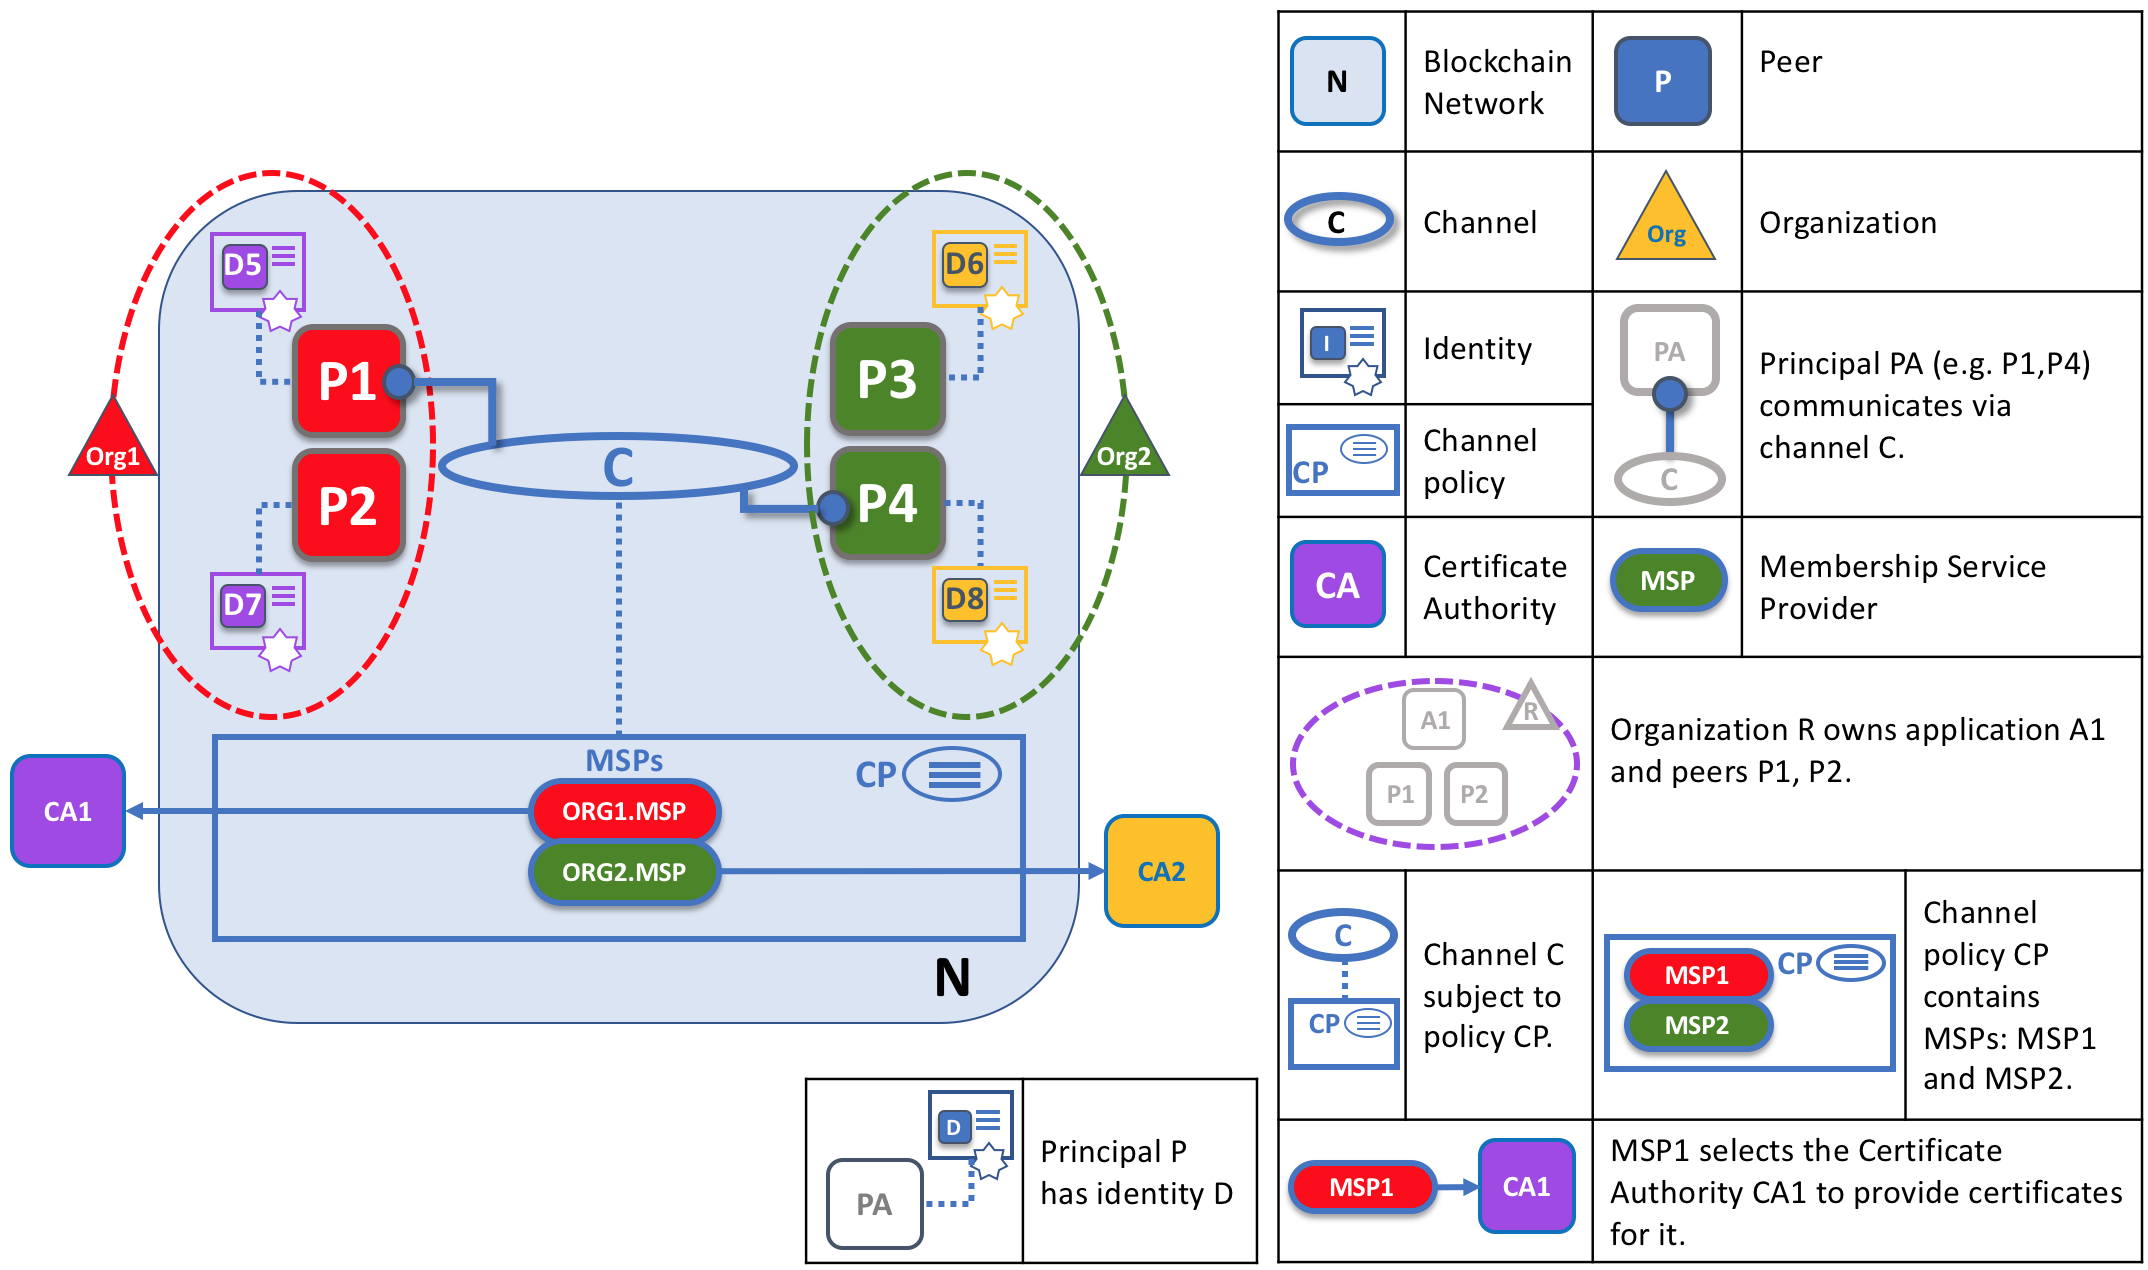
\includegraphics[scale=0.25]{recursos/orgs.png}}
\caption{Red Fabric con organizaciones y MSPs.}
\label{orgs-msp}
\end{figure}
En la figura anterior se puede observar como los \textit{peers} están dentro de organizaciones, con sus certificados correspondientes. La combinación del certificado y la identidad otorgada por el \acrshort{msp} da lugar a la identidad organizativa, denominada principal.
\subsubsection{Membership Service Providers}
Un \acrshort{msp} es el mecanismo utilizado para probar la identidad y la confianza en un actor dentro de una organización, además de otorgar roles a los participantes de la red.\\
Hay dos tipos de \acrshort{msp}s, locales y globales:
\begin{itemize}
    \item \textbf{MSP Local:} Los \acrshort{msp}s locales afectan a un nodo individualmente, y definen los permisos del mismo. Todos los nodos de la red deben tener definido un \acrshort{msp} local, ya que decide los derechos de participación a ese nivel.
    \item \textbf{MSP global:} Los \acrshort{msp}s globales controlan los derechos de participación a nivel de \textit{channel}. Todos los nodos del \textit{channel} pueden ver a los \acrshort{msp}s globales, y gracias a él pueden autenticar a todos los participantes del \textit{channel}. Todas las organizaciones que participen en un \textit{channel} deben tener un \acrshort{msp} propio, que decide que acciones pueden ejecutar los miembros en el \textit{channel}. A su vez, todos los \acrshort{msp}s de las organizaciones se incluyen en el \acrshort{msp} global.\\
    A diferencia de los \acrshort{msp}s locales, que se definen en el sistema de ficheros de cada nodo, los \acrshort{msp}s globales estan instanciados en todos los nodos del \textit{channel} y se sincronizan por consenso, de forma similar al \textit{ledger} del \textit{channel}.
\end{itemize}
\begin{figure}[H]
\centerline{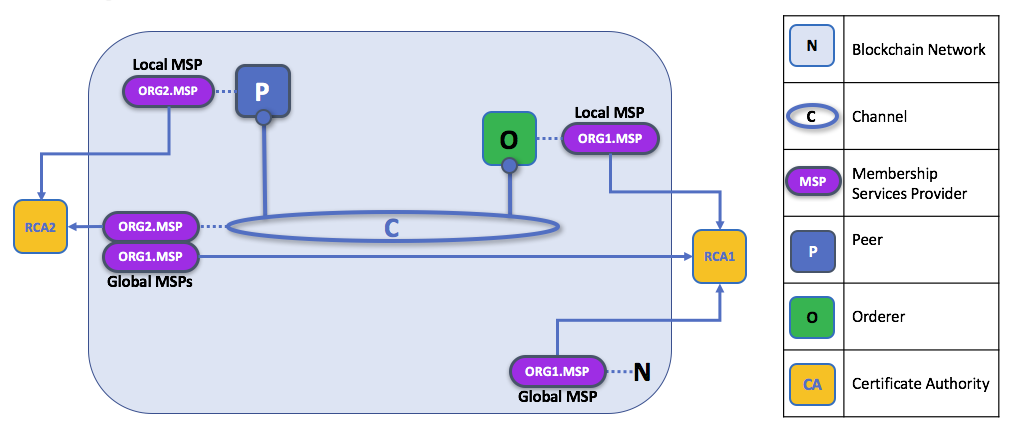
\includegraphics[scale=0.45]{recursos/msp.png}}
\caption{Red Fabric con MSPs locales y globales.}
\label{msps}
\end{figure}
En la imagen se puede observar una red típica, con un nodo de cada tipo y los \acrshort{msp} de cada organización. Estos se comunican tanto con los nodos en el canal como con las autoridades de certificación para asignar las identidades a cada miembro de la red.
\clearpage
\section{TrustOS}
Para concluir este capítulo, es interesante comentar la existencia de TrustOS, y su reciente relación con Alastria ID.
TrustOS es un conjunto de herramientas en forma de API desarrollada por Telefónica que simplifica la incorporación a una red blockchain de cualquier negocio o empresa, con diferentes módulos independientes para diferentes casos de uso, desplegados sobre redes ya existentes, y con la posibilidad de añadir APIs personalizadas o nuevos smart contracts dependiendo del caso de uso. Puede desplegarse sobre cualquier red de Hyperledger Fabric, y en el futuro también funcionará en redes Quorum y CORDA.
\begin{figure}[H]
\centerline{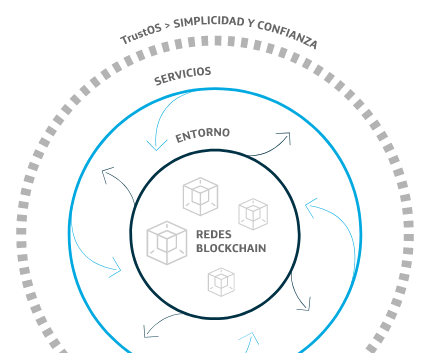
\includegraphics[scale=1]{recursos/trustos.png}}
\caption{TrustOS sobre servicios blockchain.}
\label{trustos}
\end{figure}
Funciona como una capa que encapsula los servicios blockchain, de forma que no es necesario poseer los conocimientos técnicos para incorporar funcionalidades blockchain a cualquier negocio. Se compone de cuatro módulos independientes, que disponen cada uno de un smart contract desplegado sobre varias redes blockchain, y una API para acceder comodamente a ellos. Los módulos son los siguientes:
\begin{itemize}
    \item \textbf{TRACK:} Se encarga de la representación digital de cualquier tipo de activo real, cuyo estado se monitoriza de forma transparente e inmutable, utilizando las características propias de la blockchain.
    \item \textbf{TOKEN:} Se encarga de crear ``tokens'', representaciones digitales de activos reales, dando valor real a cosas que por si solas no lo tendrían, creando la posibilidad de intercambios de activos entre empresas que confían mutuamente.
    \item \textbf{SETTLE:} Se encarga de proporcionar un sistema de consenso transparente y seguro entre los participantes, mediante el uso de smart contracts en la blockchain, para que no haya una entidad central administradora, y depositando la confianza en el propio proceso.
    \item \textbf{TRUST:} Esta relacionado con los demás módulos, y se encarga de registrar en una blockchain pública las operaciones de confianza entre miembros de la red, para crear un extra de transparencia a los procesos y garantizar la inmutabilidad de la información.
\end{itemize}
Recientemente, Inetum, un grupo empresarial estrechamente relacionado con Alastria, y Telefónica, han establecido un acuerdo para implementar el modelo Alastria ID sobre la plataforma de TrustOS, y desplegarlo en la red-H de Alastria.

\chapter{Análisis comparativo Quorum y Fabric}
\section{Redes disponibles}
Quorum es una tecnología blockchain open source creada por J.P. Morgan e implementada sobre Ethereum, que añade diferentes mejoras a la plataforma para adaptarla al mundo financiero, aunque se puede utilizar en cualquier tipo de industria. Utiliza algoritmos de consenso distintos a Ethereum, es privada y permisionada, ya que implementa control de acceso a los nodos, y tiene un rendimiento mucho mejor que Ethereum.
Hyperledger Fabric es también open source, y fue creada por IBM y Linux Foundation. Es privada y completamente modular, lo que la ha convertido en una de las opciones mas populares a la hora de implementar soluciones empresariales.\\
Ambos tipos de tecnologías tienen ventajas y desventajas a la hora de implementar Alastria ID. En los siguientes apartados se hará una comparativa entre ambas tecnologías.
\section{Casos de uso}
Ambas redes están orientadas al entorno empresarial, por lo que los casos de uso disponibles son muy similares. Sus principales puntos fuertes son la privacidad y el rendimiento, por lo que son idóneas para utilizarse como libro de cuentas o para aumentar la transparencia de las gestiones en un grupo empresarial. También son muy adecuadas para la gestión de identidad y datos personales, gracias a las características propias de la blockchain.
\clearpage
\section{Métricas tecnológicas}
En cuanto a la comparación técnica, el funcionamiento interno de ambas tecnologías es muy distinto, pero sus métricas son similares.
\subsection*{Rendimiento y consenso}
Ambas redes, al ser privadas y permisionadas, tienen un rendimiento muy alto, debido a que no necesitan algoritmos de consenso pesados. En Quorum, se utilizan \textit{RAFT}, \textit{Proof of Authority} o \textit{Istanbul BFT} como algoritmos de consenso, mucho mas rápidos que \textit{Proof of Work}, utilizado en Ethereum. En el caso de Fabric, el algoritmo por defecto es Solo, usado únicamente en entornos de prueba, aunque al ser modular, se pueden usar otros algoritmos decididos por los miembros de cada red. Los más utilizados son \textit{Kafka} y \textit{RAFT}.
En cuanto a transacciones por segundo, según estudios realizados con redes de ambas tecnologías, \cite{fabric-benchmark} \cite{quorum-benchmark} Hyperledger Fabric es capaz de conseguir un pico mas alto de rendimiento, con mas de 800 t/s, aunque con cargas de trabajo mas significativas el rendimiento puede bajar hasta a 60 t/s. En el caso de Quorum, los picos son mas bajos, de alrededor de 170 t/s, pero se mantienen mas constantes cuando aumenta la carga de trabajo. Estos rendimientos son aproximados, y dependen en gran medida del algoritmo de consenso utilizado, las características de la red, o en el caso de Fabric, el tipo de base de datos que se utilice para el \textit{world state}.
\clearpage
\subsection*{Smart Contracts}
En lo referente a los smart contracts, hay algunas diferencias entre Quorum y Fabric, pero en general son muy similares. Los smart contracts son la lógica de negocio que se ejecuta en la blockchain y la actualiza, y dependiendo de la red, hay diferentes métodos de despliegue. En Quorum, cualquier nodo autorizado puede desplegar un smart contract en la red. \\
\begin{figure}[H]
\centerline{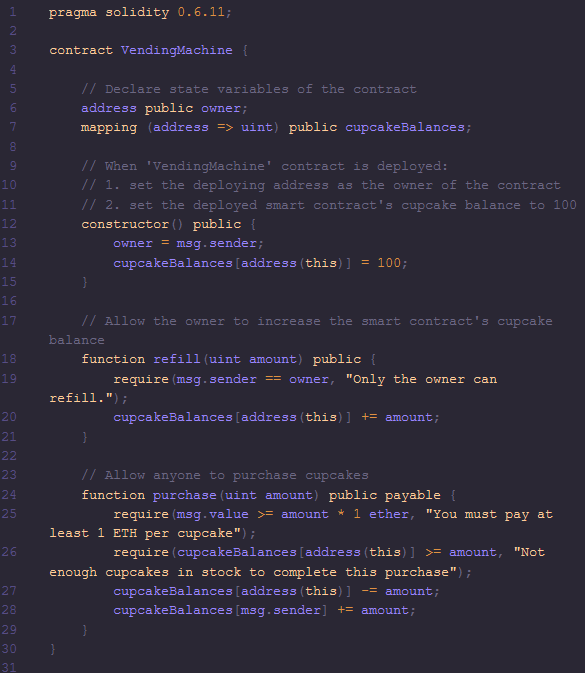
\includegraphics[scale=0.85]{recursos/smartcontracteth.png}}
\caption{Smart contract en Solidity para Ethereum \cite{SC-ETH}}
\label{sc-eth}
\end{figure}
En la imagen se puede observar un código bastante simple que permite el intercambio de ``cupcakes'' virtuales a cambio de ETH. Al ser Quorum una implementación de Ethereum, se utiliza el lenguaje Solidity para la codificación de los smart contracts de ambas tecnologías.\\

En Fabric, son las organizaciones las que despliegan el código en la red, y son las que se encargan de decidir la política de aprobación (\textit{endorsement policy}) de cada smart contract. La política de aprobación es una lista de las organizaciones cuya validación se requiere para aprobar una transacción creada por un smart contract en particular.
\begin{figure}[H]
\centerline{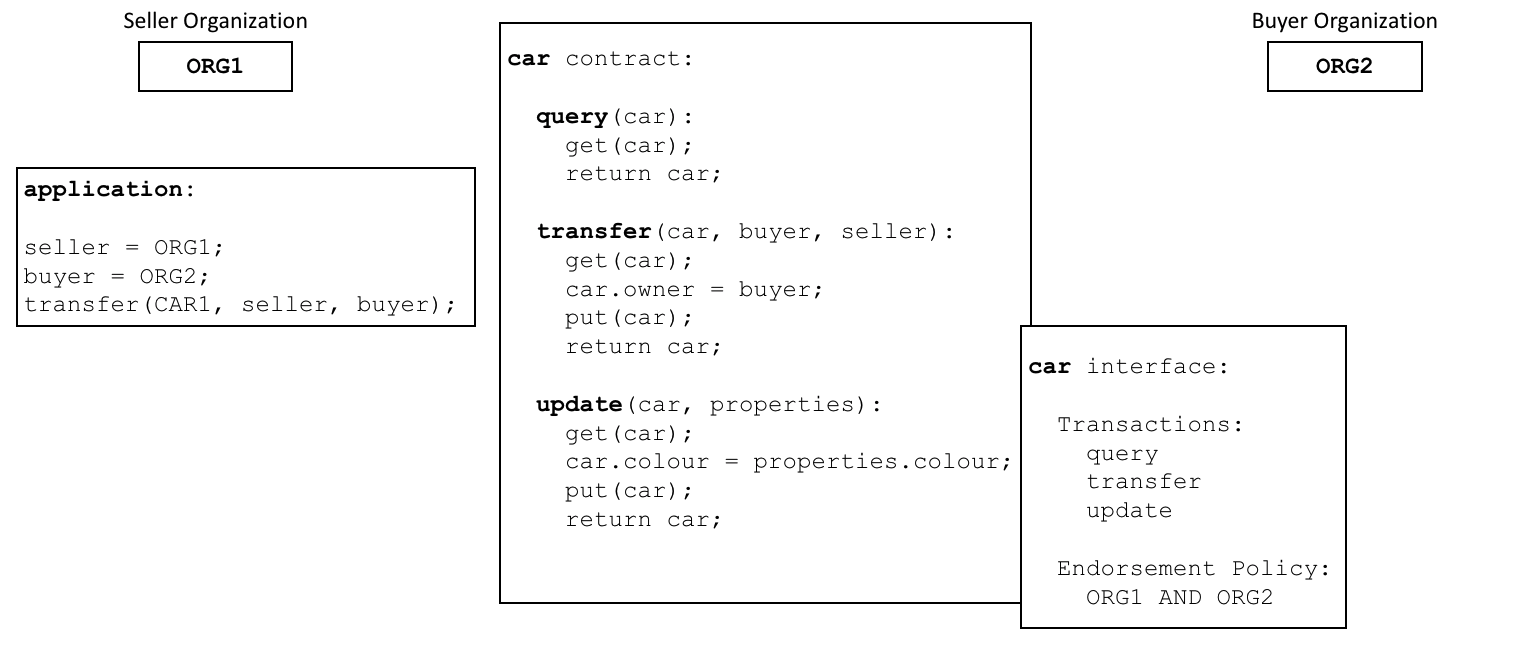
\includegraphics[scale=0.35]{recursos/SC-FABRIC-END.png}}
\caption{Smart contract de Fabric \cite{chaincodes}}
\label{sc-fabric}
\end{figure}
En la imagen se puede observar un código de un simple intercambio de objetos o \textit{assets}, con dos organizaciones involucradas, junto con su política de aprobación. Está escrito en pseudocódigo porque los smart contracts de Fabric no tienen un lenguaje único, sino que se pueden escribir en distintos lenguajes de propósito general, como Node.js o Go, lo que facilita el trabajo a desarrolladores ya experimentados. Abajo a la derecha se puede observar la política de aprobación del smart contract, que indica que organizaciones deben firmar las transacciones creadas por el smart contract para que sean válidas y puedan actualizar el world state.

Una diferencia importante entre los smart contracts de Quorum y los chaincodes de Fabric es su forma de desplegarse.
En Quorum, los smart contracts tienen su propia dirección en la red, y se comportan como un elemento más de la misma. Además, almacenan los datos en estructuras de datos implementadas en el propio código (un ejemplo es el \textit{mapping} ``cupcakeBalance'' de la figura \ref{sc-eth}). Debido a estas dos características, actualizar o mejorar el código de un smart contract desplegado es imposible, y se debe desplegar de nuevo como un contrato distinto, perdiendo asi los datos almacenados en el smart contract y cambiando su dirección. Este problema se puede solucionar con los llamados \textit{upgradeable contracts}, que permiten actualizar su código sin tener que desplegarlos de nuevo. En la implementación actual de Alastria ID para la red-T, los smart contracts no son actualizables, aunque su implementación esta en proceso.

En Fabric, los smart contracts no se despliegan por si solos, sino que se empaquetan en los chaincodes, que cada organización tiene que desplegar y aprobar para su activación en la red (por ejemplo, el smart contract de la figura \ref{sc-fabric} podría formar parte de un chaincode de vehículos mayor, con otros smart contracts como ``barco'' o ``motocicleta''). Las redes Fabric, al utilizar una base de datos de estados para almacenar los datos, no tienen problemas de perdida de información a la hora de actualizar o mejorar un chaincode, y solo con desplegar la nueva versión en la red todos los nodos involucrados apuntarán al chaincode mas actualizado.
 

\chapter{Alastria ID}
En los siguientes apartados se mostrará la implementación actual de los contratos en la red Quorum y se describirá un posible diseño para las redes Fabric.
\section{Arquitectura en Ethereum}
\subsection{Smart Contracts}
La implementación Quorum de Alastria ID está dividida en tres grupos de smart contracts, cada uno encargado de una función del modelo. Estos smart contracts actualmente están desplegados en la red-T de Alastria.
\begin{figure}[H]
\centerline{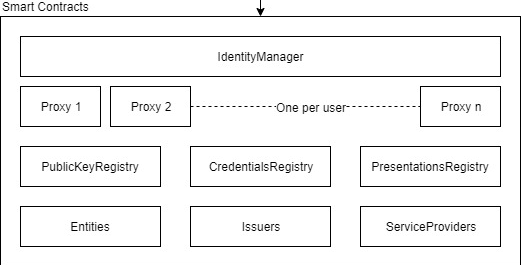
\includegraphics[scale=1]{recursos/alastriaid-sc.png}}
\caption{Estructura smart contracts de AlastriaID en Solidity.}
\label{sc-alastriaeth}
\end{figure}
\subsubsection{Gestión de identidad}
Los contratos de este grupo se encargan de la creación de identidades y el envío de transacciones.
\begin{enumerate}
    \item \textbf{AlastriaIdentityManager.sol:} Genera tokens de acceso, crea identidades creando un AlastriaProxy por cada una y envía transacciones a través de dichos proxies.
    \item \textbf{AlastriaProxy.sol:} Es la identidad en si. Cada Alastria ID tiene un proxy y este es el que se encarga de reenviar las transacciones. Todas las transacciones le llegan desde el AlastriaIdentityManager.
    \item \textbf{AlastriaIdentityIssuer.sol:} Es el encargado de registrar las identidades de los issuers.
    \item \textbf{AlastriaIdentityServiceProvider.sol:} Es el encargado de registrar las identidades de los service providers.
    \item \textbf{AlastriaIdentityEntity.sol:} Es el encargado de registrar todas las entidades.
\end{enumerate}
\subsubsection{Registro}
Los contratos de este grupo se encargan de almacenar toda la información sobre la transferencia de credenciales.
\begin{enumerate}
    \item \textbf{AlastriaCredentialRegistry.sol:} Se encarga de almacenar todas las credenciales y su estado. El estado de una credencial define si su uso es posible o ha sido revocada. Hay cuatro estados posibles:
    \begin{enumerate}
        \item \textbf{Estado 0/Valid:} Significa que la credencial es válida y esta lista para su uso.
        \item \textbf{Estado 1/AskIssuer:} Una credencial puede estar en este estado tras ser emitida, significa que debemos preguntarle al issuer sobre su validez.
        \item \textbf{Estado 2/Revoked:} Significa que el issuer ha revocado el uso de la credencial.
        \item \textbf{Estado 3/DeletedBySubject:} Significa que el sujeto ha decidido no permitir mas el uso de la credencial y quiere que se elimine.
    \end{enumerate}
    \item \textbf{AlastriaPresentationRegistry.sol:} Se encarga de almacenar todas las presentations y su estado. El estado de una presentation define si su uso es posible. Hay cuatro estados posibles:
    \begin{enumerate}
        \item \textbf{Estado 0/Valid:} Estado inicial de la presentation cuando es emitida por el subject.
        \item \textbf{Estado 1/Received:} Significa que el service provider ha recibido la presentation del subject.
        \item \textbf{Estado 2/AskDeletion:} Significa que el subject ha decidido revocar la presentation y que no se usen las credenciales que contiene.
        \item \textbf{Estado 3/DeletionConfirmation:} Estado que se alcanza cuando el service provider confirma el borrado solicitado a través del estado 2.
    \end{enumerate}
    \item \textbf{AlastriaPublicKeyRegistry.sol:} Se encarga de almacenar todas las claves públicas.
\end{enumerate}
\subsubsection{Librerias}
Por último, los smart contracts hacen uso de dos librerias auxiliares.
\begin{enumerate}
    \item \textbf{Eidas.sol:} Se utiliza para gestionar los \acrshort{loa} de las credenciales.
    \item \textbf{Owned.sol:} Se utiliza para asegurar que el acceso a un solo lo realiza la cuenta que lo creó. Es una librería muy común en proyectos Solidity.
\end{enumerate}
\section{Arquitectura en Fabric}
\subsection{Chaincode}
Mi propuesta de implementación en Fabric de Alastria ID esta dividida en tres paquetes de smart contracts y un contrato aparte que encapsula su contexto de transacciones. Este conjunto de smart contracts está codificado en Go, y se empaqueta para formar un chaincode.
\subsubsection{API Ledger}
Los contratos de este grupo son una API diseñada para interactuar de manera mas cómoda con el ledger.
\begin{enumerate}
    \item \textbf{state.go:} Se encarga de crear Keys para normalizar el almacenamiento de todos los datos en el ledger.
    \item \textbf{stateList.go:} Se encarga de todos los accesos al ledger, tanto de lectura como escritura, utilizando las Keys creadas con \textbf{state.go}.
\end{enumerate}
\subsubsection{Gestión de identidad}
Los contratos de este grupo se encargan de la creación de identidades, sobre todo para las entidades.
\begin{enumerate}
    \item \textbf{entity.go:} Se encarga de la especificación de entidades, ya sean issuer, service provider o ninguna de las dos.
    \item \textbf{entityList.go:} Se encarga de encapsular \textbf{stateList.go}, adaptándolo al almacenamiento de entidades.
    \item \textbf{entityContract.go:} Se encarga de la lógica para la gestión y creación de entidades, así como de la asignación de roles a las mismas.
    \item \textbf{identity.go:} Se encarga de la especificación de identidades de sujeto o de entidad.
    \item \textbf{identityList.go:}  Se encarga de encapsular \textbf{stateList.go}, adaptándolo al almacenamiento de identidades de todo tipo.
    \item \textbf{identityContract.go:} Se encarga del almacenamiento y la creación de identidades de sujetos.
    \item \textbf{identityContext.go:} Se encarga de encapsular TransactionContextInterface y de compartir el contexto de transacciones entre todos los contratos de gestión de identidad, añadiendo las stateList de todos ellos al mismo.
\end{enumerate}
\subsubsection{Registro}
Los contratos de este grupo se encargan de la gestión y registro de credenciales y presentaciones.
\begin{enumerate}
    \item \textbf{credential.go:} Se encarga de la especificación de credenciales, ya sean tipo subject o issuer.
    \item \textbf{presentation.go:} Se encarga de la especificación de presentaciones, ya sean tipo subject o receiver.
    \item \textbf{credentialList.go:} Se encarga de encapsular \textbf{stateList.go}, adaptándolo al almacenamiento de credenciales.
    \item \textbf{presentationList.go:} Se encarga de encapsular \textbf{stateList.go}, adaptándolo al almacenamiento de presentaciones.
    \item \textbf{credentialContract.go:} Se encarga de la lógica para la gestión y creación de credenciales.
    \item \textbf{presentationContract.go:} Se encarga de la lógica para la gestión y creación de presentaciones.
    \item \textbf{registryContext.go:} Se encarga de encapsular TransactionContextInterface y de compartir el contexto de transacciones entre todos los contratos del registro, añadiendo las stateList de todos ellos al mismo.
\end{enumerate}

En la raíz del proyecto, se encuentra un archivo más, \textbf{main.go}, que se encarga de inicializar los chaincodes.

\clearpage

\section{Comparativa}
El funcionamiento de los smart contracts tanto en Solidity como en Go es muy similar, con algunas diferencias debido al lenguaje de programación y a la naturaleza de la red.

En cuanto al registro de credenciales y presentaciones, el funcionamiento es idéntico, salvo que en Fabric se hace uso del \textit{world state} para almacenar los datos. Además, debido a que la identidad en Fabric se gestiona a nivel de red, y que no es posible el uso de los AlastriaProxies, no se ha considerado necesario implementar el contrato AlastriaPublicKeyRegistry, que gestiona y almacena las claves públicas.

En lo respectivo a los contratos de gestión de identidad y entidades, se han eliminado los contratos de gestión de proveedores de servicio y emisores, y se han centralizado en un contrato de gestión de entidades en general. En los nuevos contratos, todas las entidades se guardan de la misma forma en el \textit{world state}, y se diferencian entre ellas mediante atributos.

Se ha incluido un contrato equivalente a AlastriaIdentityManager.sol, con funcionamiento similar, salvo por el uso de proxies, que no existen en la implementación de Fabric. Esto es un problema importante, puesto que solo sería posible crear un AlastriaID por cada sujeto, ni implementar la función de recuperación de cuentas.

En la implementación de Fabric se utilizan algunas librerías de utilidades y se implementa la API de Fabric para interactuar con los nodos de la red, y además, se han creado dos contratos auxiliares que definen un tipo de listas y objetos que permiten interactuar mas cómodamente con el \textit{ledger}, y que se implementan en múltiples contratos, tanto de registro como de identidad. También hay un contrato extra que encapsula el contexto de transacciones y lo comparte entre todos los demás, para que sea posible compartir la información entre todos ellos dentro del chaincode.

Por último, como en Fabric todos los smart contracts se despliegan a la vez, se han dividido lo mas posible para mejorar su comprensibilidad.


\chapter{Implementación en Fabric}
\section{Diseño}
\subsection{Registro}
Debido a que en Fabric se utiliza una base de datos (\textit{world state}) para almacenar datos, no es necesario crear estructuras de datos en memoria para guardar las credenciales y las presentaciones. Ambas se crean en formato clave-valor, utilizando su \acrshort{psmhash} como clave y un objeto JSON con toda la información relevante como valor. Solo se utiliza un objeto credencial, y se diferencia entre credenciales de emisor o de sujeto mediante un campo ``type'' en el JSON de cada credencial.

\begin{figure}[H]
\centerline{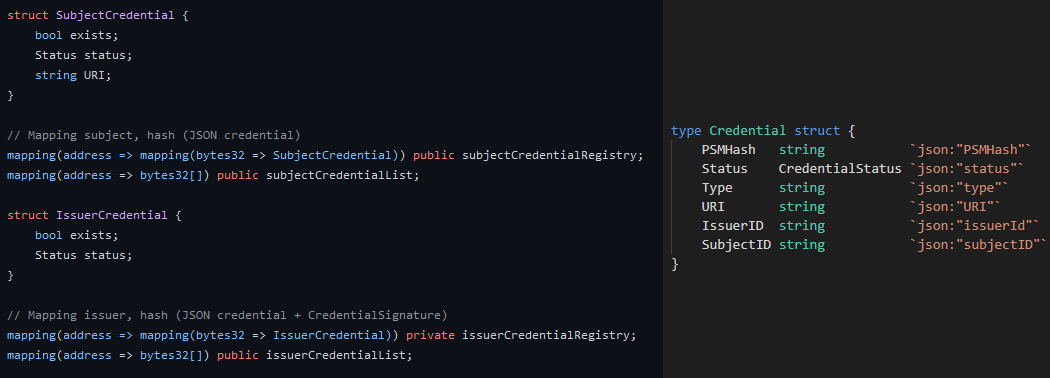
\includegraphics[scale=0.55]{recursos/subjectcredential.png}}
\caption{Comparación Credential entre Solidity y Go.}
\label{credential-comp}
\end{figure}
En la imagen a la izquierda está la implementación en Solidity y a la derecha en Go, se puede observar que en Go solo se utiliza un objeto para todo tipo de credenciales, y que no se utilizan mappings para almacenarlas, ya que en Fabric los datos se guardan en el \textit{world state}. Los campos específicos de las credenciales de sujeto se quedaran vacíos en las de emisor, y viceversa.

\begin{figure}[H]
\centerline{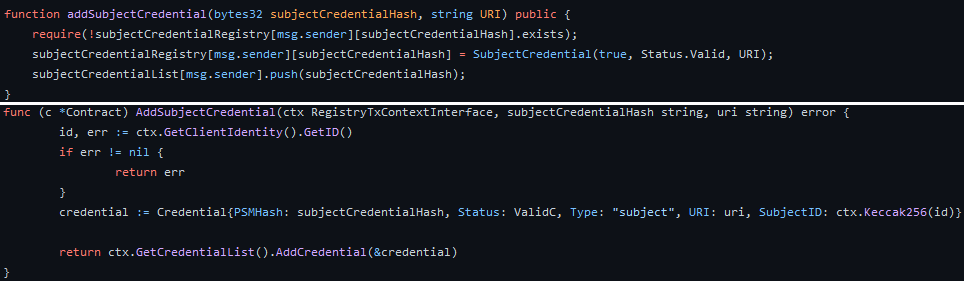
\includegraphics[scale=0.60]{recursos/addsubjectcredential.png}}
\caption{Comparación de la función addSubjectCredential entre Solidity y Go.}
\label{add-credential-comp}
\end{figure}
En la imagen arriba está la implementación en Solidity y abajo en Go de la función ``AddSubjectCredential'', para añadir credenciales de sujeto. Como se puede observar, en Go se crea un objeto JSON con los datos y se guarda en el \textit{world state}, rellenando en este caso el campo SubjectID con el ClientID del llamante hasheado con keccak256. Se ha optado por esta función de hash para que sea lo mas similar posible a la implementación Solidity, pero se podrían utilizar otros algoritmos. La función ``AddIssuerCredential'', que sirve para añadir credenciales de emisor, sería identica, salvo por que en el objeto credencial se rellenaría el campo IssuerID y se dejaría el campo URI vacío.

En el caso de las presentaciones el funcionamiento es prácticamente idéntico, con un solo objeto presentación y un campo ``type'' para diferenciar entre sujeto y receptor.
\subsection{Identidad}
En lo referente a entidades, se eliminan los objetos de emisor y proveedor de servicios, y se concentran en un objeto Entity, que se define como uno u otro mediante atributos booleanos ``isIssuer'' e ``isServiceProvider''. Esto además soluciona el problema de que una entidad pudiera tener un rol sin ser técnicamente ``entity''.
\begin{figure}[H]
\centerline{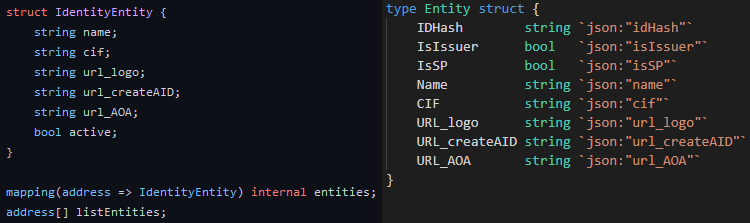
\includegraphics[scale=0.8]{recursos/entities.png}}
\caption{Comparación Entity entre Solidity y Go.}
\label{entities-comp}
\end{figure}
En la imagen a la izquierda esta la implementación en Solidity y a la derecha en Go del objeto Entity. En la implementación en Solidity, este objeto solo contiene la información sobre la entidad, pero para almacenar entidades emisoras o proveedoras de servicio utiliza otras estructuras, repartidas en dos smart contracts. En Go, se elimina la necesidad de estos dos smart contracts y se concentran las entidades en un solo objeto, que tiene los mismos campos que en Solidity más tres campos extra que indican el rol de la entidad y la identidad que le corresponde. Una vez más, no es necesario el mapping en Go ya que los datos se almacenan en el \textit{world state}.

En Quorum, cada entidad está representada por una dirección propia y fácilmente manejable. En Fabric, cada entidad representaría a una organización, pero como las organizaciones no tienen un certificado propio ni nada que las identifique como tal, se utilizaría una identidad estándar para representar a cada entidad/organización, y cada una de ellas accedería a la blockchain como si fuera un sujeto, a través de un wallet de identidad. Dentro de los chaincodes es donde se reconocería a cada identidad como entidad o sujeto. 

En la implementación de Solidity existe un problema con los nuevos despliegues, y es que se necesita una primera entidad emisora para poder empezar a crear identidades. La antigua solución era crear la primera entidad a mano utilizando la cuenta de administrador, pero con los nuevos smart contracts en desarrollo, el problema se soluciona mediante un parámetro pasado en la inicialización de los contratos. En Fabric surge el mismo problema, pero se puede aplicar la misma solución que en Solidity, creando esa primera entidad en la inicialización del chaincode.

Todo el funcionamiento de la entidad, ya sea emisora, proveedora de servicios, o ninguna de los dos, se ha concentrado en un solo smart contract, que realizará todas las gestiones pertinentes.

En cuanto a la creación de identidades, se eliminan los AlastriaProxy, pero el resto del funcionamiento se mantiene similar. Las identidades se almacenan como un objeto JSON con tres atributos.
\begin{figure}[H]
\centerline{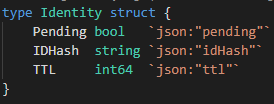
\includegraphics[scale=1]{recursos/identity.png}}
\caption{Objeto JSON que representa las identidades.}
\label{identity-json}
\end{figure}
\begin{itemize}
    \item \textbf{Pending:} Booleano que se activa cuando un emisor inicia el proceso de creación de la identidad. Es el equivalente a la función ``prepareAlastriaID'' en los contratos en Solidity.
    \item \textbf{IDHash:} String que representa el identificador de la identidad. En la implementación en Solidity se utiliza la dirección del AlastriaProxy correspondiente, pero como en este modelo no existen los proxies, se utiliza un hash keccak256 del ClientID del sujeto al que se le va a crear la identidad.
    \item \textbf{TTL:} Time To Live. Tiempo en formato UNIX que no se debe haber superado a la hora de crear la identidad.
\end{itemize}
Debido a que no es posible el uso de proxies, la creación de AlastriaIDs quedaría limitada a uno por ClientID, a diferencia de la implementación en Solidity. Puesto que no se puede crear mas de una identidad por sujeto, no se puede implementar la función de recuperación de cuentas.

Respecto a la creación de identidades y los IDHashes, una alternativa sería que la propia organización ya almacenase los ClientID en formato hash, así no haría falta hashearlos en el propio chaincode.

\section{Implementación}
La implementación de los smart contracts para la red Fabric está hecha en Go, y la base de datos que se utiliza para el world state es LevelDB, para cuyas búsquedas se crean claves compuestas con la información relevante. Otra opción sería usar CouchDB, que permite la búsqueda por valor y no solo por clave, lo que facilita mucho las búsquedas, aunque requiere cambiar configuración de la red y preestablecer unos índices que, de crecer mucho, podrían afectar al rendimiento de la red. Todos los hashes utilizan la función Keccak256, para mantener el paralelismo con la implementación en Solidity, aunque se podrían usar otras funciones de hash si así se quisiese.\\

La red utilizada es la red de pruebas facilitada en el GitHub oficial de Fabric, con utilidades para desplegar rápidamente una red con dos organizaciones y todos los nodos necesarios para desplegar chaincodes inmediatamente. Los nodos se despliegan mediante contenedores Docker, así como los chaincodes. Aun así, los chaincodes podrían desplegarse en cualquier red Fabric.
\begin{figure}[H]
\centerline{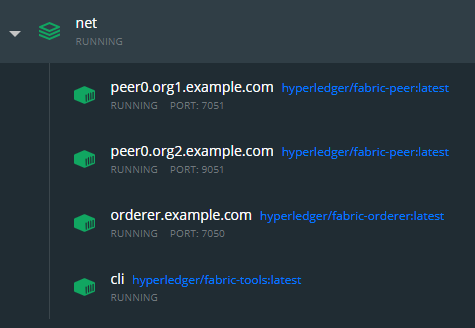
\includegraphics[scale=0.9]{recursos/network-daocker.png}}
\caption{Contenedores Docker con los nodos de la red.}
\label{docker-net}
\end{figure}
En la imagen se puede observar la red Docker de pruebas, con un \textit{peer} por organización y un \textit{orderer} común. El contenedor CLI es la consola de Fabric. Los chaincodes se despliegan en contenedores independientes.

\begin{figure}[H]
\centerline{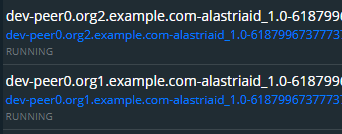
\includegraphics[scale=0.9]{recursos/chaincodes-docker.png}}
\caption{Contenedores Docker con los chaincodes.}
\label{chaincodes-docker}
\end{figure}
En la imagen se pueden observar dos contenedores, pero contienen el mismo chaincode, porque cada organización lo despliega independientemente después de llegar a un acuerdo.

Las identidades se han generado utilizando la herramienta Cryptogen, diseñada solo para entornos de pruebas. En una red real las identidades son gestionadas por las autoridades de certificación (CA), organizaciones que emiten certificados e identidades digitales. 

Por falta de tiempo, solo se ha realizado la implementación del grupo \textbf{API Ledger}, de \textbf{identityManager.go}, y de los contratos de gestión de credenciales.

\chapter{Análisis de impacto y desafíos}
En este capítulo se realizará un análisis del impacto potencial de los resultados obtenidos durante la realización del TFG, en los diferentes contextos para los que se aplique.
\section{Impacto potencial}
\subsection{Personal}
En el ámbito personal, la realización de este trabajo me ha supuesto un desafío a la hora de investigar sobre nuevas tecnologías, ya que he tenido que aprender de cero prácticamente todo con lo que he trabajado para el proyecto. También ha supuesto un reto el adaptar un modelo existente a una tecnología que no es del todo compatible con el mismo.\\
La parte mas complicada ha sido el aprendizaje de Hyperledger Fabric, ya que ha resultado ser una tecnología mucho mas compleja de lo esperado. Por otro lado, la parte mas sencilla de aprender ha sido Alastria ID, debido a que ya estaba familiarizado con el modelo y solo he tenido que profundizar en los smart contracts.
\subsection{Empresarial}
Tanto Quorum como Hyperledger Fabric están diseñadas con el aspecto empresarial en mente, y ambas tienen casos de uso que pueden aportar mucho valor a empresas de cualquier industria. La implementación de Alastria ID en una red más ampliaría el abanico de opciones que tendrían las empresas interesadas en soluciones de este tipo, pudiendo elegir la red mas apropiada a sus circunstancias.
\clearpage
\section{Objetivos de desarrollo sostenible}
Este proyecto se amolda sobre todo al objetivo número 9, sobre industria, innovación e infraestructuras. Sólo en España, un 96\% de personas utilizan teléfono móvil, y un 91\% tiene acceso a internet, por lo que la adopción del modelo Alastria ID en la sociedad actual conllevaría un gran avance en los sistemas de provisión de servicio, y en la gestión de los datos personales de cualquier individuo. Además, en el ámbito empresarial, incorporar el modelo aceleraría todo tipo de procesos de negocio, y aumentaría la confianza y la transparencia a la hora de realizar servicios, tanto en la empresa pública como en el sector privado.

También se ajusta al objetivo 13, de acción por el clima, ya que si se sustituye el uso de credenciales físicas o en papel por credenciales digitales, se reduce la contaminación y la producción de tarjetas, documentos, etc..., que son perjudiciales para el planeta.

Gracias a las credenciales digitales, el modelo podría adaptarse también al resto de objetivos. Por ejemplo, los objetivos 1 y 2, fin de la pobreza y hambre cero, se podrían cubrir con una credencial de vulnerabilidad económica, que podría acreditar a una familia para recibir ayudas del estado, o el objetivo 3, salud y bienestar, se podría cumplimentar con una credencial PCR, para acreditar un negativo ante pruebas COVID. La identidad digital proporcionada por el modelo de Alastria ID es un concepto transversal que, utilizada correctamente, puede ayudar a cumplir todos los objetivos de desarrollo sostenible.

\chapter{Resultados y conclusiones}
\section{Resultados y líneas futuras}
Tras la realización de este trabajo, se ha diseñado un chaincode para Alastria ID que implementa parcialmente su funcionalidad, debido a ciertos problemas que surgen debido a las características de la red. Sin embargo, con más investigación es muy probable que se puedan solucionar. Tanto las redes de Fabric como las de Quorum comparten muchas características que las hacen viables para este tipo de soluciones, y es decisión del usuario utilizar una u otra, ya que en cuanto a rendimiento son muy similares.

Como trabajo futuro, hay varios puntos en los que se puede trabajar:
\begin{itemize}
    \item \textbf{Implementación de SC restantes:} Como se ha mencionado anteriormente, para este trabajo solo se han implementado ciertos smart contracts, así que un punto de continuidad sería terminar toda la implementación.
    \item \textbf{Creación de identidades:} Debido a la incompatibilidad de los Alastria Proxies con Fabric, hay funcionalidades que no se pueden implementar con facilidad. Para ello, se podrían utilizar atributos de los certificados X.509 para crear las identidades de Alastria. Sería necesario para poder crear mas de un AlastriaID por ClientID y para poder implementar la función de recuperación de cuentas.
    \item \textbf{Cifrado mas ligero:} Una posible mejora sería utilizar una implementación mas ligera de las funciones para el cifrado Keccak256, porque actualmente se utiliza una librería mas grande de lo necesario.
    \item \textbf{Emisión de eventos:} Actualmente no está implementada la emisión de eventos, y es una parte muy importante de los contratos de Solidity, así que se podría investigar.
    \item \textbf{CouchDB:} Se podría usar CouchDB, que utiliza índices para guardar datos y que luego se puedan recuperar de forma mucho mas fácil, con consultas típicas de base de datos. Habría que cambiar configuración de la propia red para usar esta base de datos.
\end{itemize}
\clearpage
\section{Conclusión}
Como conclusión personal, gracias a este trabajo he podido aprender mucho sobre la tecnología blockchain, que creo que tiene un potencial inmenso, y mas en concreto sobre Hyperledger Fabric, una tecnología compleja pero con muchas capacidades. He realizado este trabajo mientras trabajaba en el equipo blockchain de una gran empresa, donde he podido conocer buenos profesionales que me han ayudado mucho a aprender sobre la tecnología. Además, he podido profundizar en el modelo Alastria ID y en la identidad digital soberana, un concepto apasionante para mi y que puede revolucionar muchos aspectos de la sociedad actual.


%%-----------------------------------------------
%% Anexos
\appendix
\clearpage 
%%---------------------------------------------------------

\newpage
\addcontentsline{toc}{chapter}{Bibliografía}

\printbibliography

\end{document}
